\documentclass[12pt, a4paper]{article}
\usepackage[utf8]{inputenc}
%\usepackage[latin1]{inputenc} 
\usepackage[english]{babel} 
\usepackage[T1]{fontenc} 
\usepackage{amsmath,amssymb} 
\usepackage[table]{xcolor}
\usepackage{verbatim}
\usepackage{graphicx}
\usepackage{fancyhdr}
\usepackage{wrapfig}
\usepackage{gauss}
\usepackage{xfrac}
\usepackage[page]{totalcount}
\usepackage{caption}
\usepackage{subcaption}
\usepackage{booktabs}
\usepackage{setspace}
\usepackage{enumitem}
\usepackage{placeins}
\usepackage{hyperref}
\usepackage{titlesec}
\usepackage{multirow}
\usepackage{epigraph}

\usepackage{multicol}

\setlength{\headheight}{15pt}

\titlespacing\section{0pt}{12pt plus 4pt minus 2pt}{0pt plus 2pt minus 2pt}
%\setcounter{tocdepth}{3}
%\setcounter{secnumdepth}{3}
%\setcounter{secnumdepth}{0}

%marginer
\usepackage[top=2.5cm, bottom=2.5cm, left=2.5cm, right=2.5cm]{geometry}


% patch gauss macros for doing their work in `align'
% and other amsmath environments; see
% http://tex.stackexchange.com/questions/146532/
\usepackage{etoolbox}
\makeatletter
\patchcmd\g@matrix
 {\vbox\bgroup}
 {\vbox\bgroup\normalbaselines}% restore the standard baselineskip
 {}{}
\makeatother
\newcommand{\BAR}{%
  \hspace{-\arraycolsep}%
  \strut\vrule % the `\vrule` is as high and deep as a strut
  \hspace{-\arraycolsep}%
}

\pagestyle{fancy}

%subsections get indexed with letters
%\renewcommand{\thesubsection}{\thesection.\alph{subsection}}

%Navn og dato
\lhead{Economics of Education}
\chead{University of Copenhagen}
\rhead{\today}

\cfoot{Page \thepage\ of \totalpages}


%begynd dokumentet
\begin{document}
%\begin{spacing}{1.213}



\title{ Economics of Education  \\ \Large Course notes \\ \normalsize \today \\ 
%\normalsize {No. of signs: }
} 
\author{\normalsize Kristian Urup Olesen Larsen}
\date{} % Use current date.
\maketitle % Print title page.
\pagenumbering{roman} % Roman page number for toc
\setcounter{page}{1} % Make it start with "ii"

%\chapter{A Main Heading} % Make a "chapter" heading
\pagenumbering{arabic} % Start text with arabic 1

%---------------------------------------------------------------
%-------SKRIV HERUNDER----------------------------------
%---------------------------------------------------------------

\epigraph{"[The] study of how individuals and society choose
with or without money,
to employ scarce productive resources
to produce various types of knowledge, skill, mind, character
over time
and distribute them, now and in the future,
among various people and groups in society."}{\textit{Elchanan, Cohn (1979)}}
\tableofcontents
\pagebreak

\begin{multicols}{2}
\section{Part 1 - math}
\subsection{Lecture 1}
This lecture introduces the course, and presents stylized facts about economics of education.

In the last 30-40 years women have been gaining more education than men, thus shifting the relative educational level from men getting the most education to women now being most educated. 
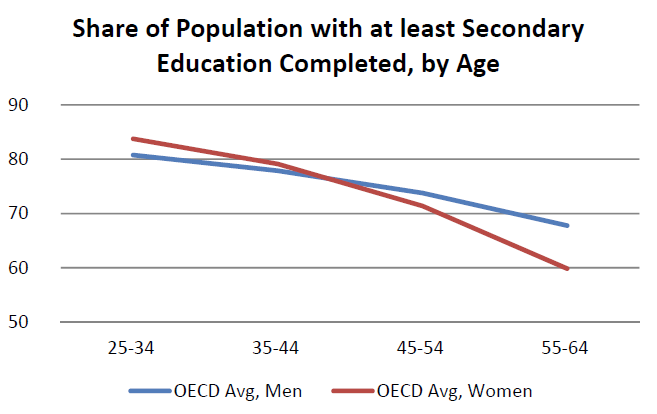
\includegraphics[width = 0.45\textwidth]{MFrates.PNG}

The private and public costs vary significantly from nation to nation.
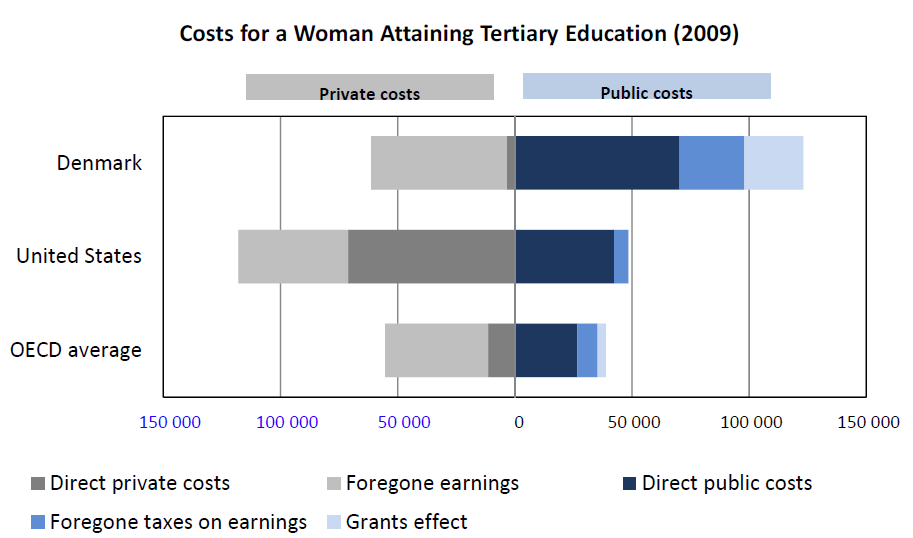
\includegraphics[width = 0.45\textwidth]{Capture.PNG}

Public costs and benefits are also very different from nation to nation, with Denmark having abnormally large public costs compared to the benefits. 
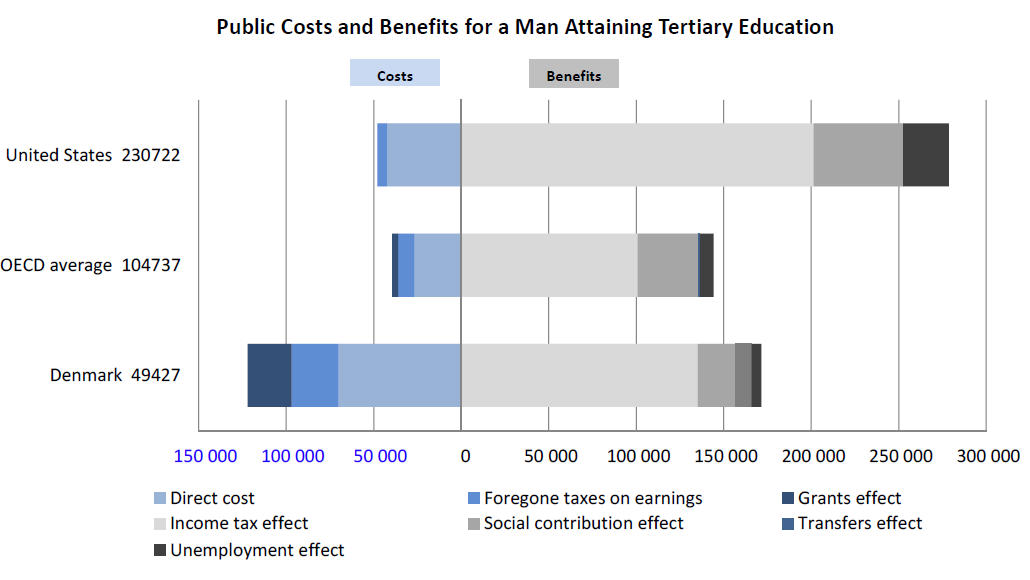
\includegraphics[width = 0.45\textwidth]{costben.PNG}

Obesity rates are declining in education for all educated countries, with th US being the only exception when comparing lower grades of education.
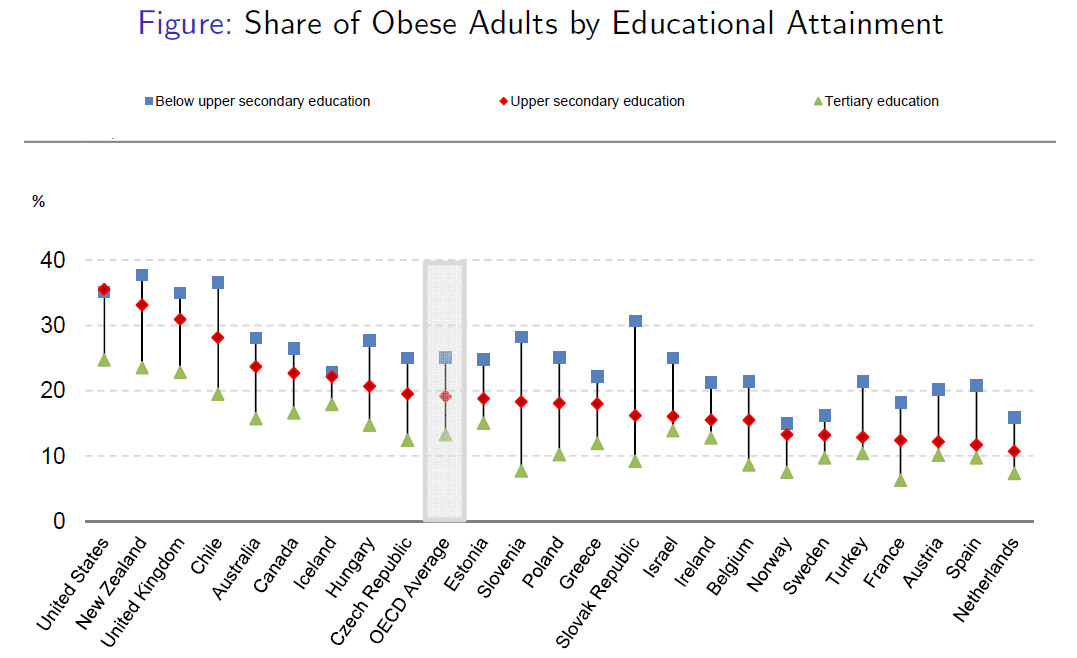
\includegraphics[width = 0.45\textwidth]{obese.PNG}

Additionally the Kuhn-Tucker theorem of constrained optimization is run through.

\subsection{Lecture 2 - Ben Porath}
Since WWII educational attainment has increased drastically, but yet large differences exist between countries. Countries with high educational attainment generally have lower differences within its borders. Importantly we do not see any decline in inequality with increases in education, yet highly educated countries are generally more equal.

\paragraph{Human capital}
Is comparable to regular capital, but distinct in that 
\begin{itemize}
\item it cannot be resold 
\item is invisible 
\item is irreversible
\item requires the investment of both time and money to obtain
\end{itemize}
Further it cannot be collateralized, and have distinct issues with information asymmetry and moral hazard.

\subsubsection{the Ben-Porath model}
There are $n$ individuals, who live over youth $t$ and adulthood $t+1$. They can choose a homogenous good $H_{ij}, j \in \{t,t+1\}$ of human capital. The labor market rewards HC with its marginal productivity $\beta_{t}$ so earnings are 
\begin{align*}
W_{ij}(H_{ij}) = \beta_j H_{ij}, \quad j\in \{t,t+1\}
\end{align*}
Human capital evolves according to
\begin{align*}
H_{it+1} = H_{it}(1-\delta) + \Delta H_{it}
\end{align*}
where we define 
\begin{align*}
\Delta H_{it} = (A_i E_{it} S_{it} H_{it})^{\alpha}, \quad \alpha<1
\end{align*}
$A$ is innate ablility, $E$ is expenditures, $S$ is schooling and $H$ is previous human capital. The discounted value of lifetime earnings $V_i$ is given the potential earnings $\beta_tH_{it}$, less the opportunity cost of schooling $S_{it}\beta_tH_{it}$ and less the direct cost of schooling $\gamma_t S_{it}$, discounted with $\rho$ over the 2 periods. So 
\begin{align*}
V_i &= \beta_tH_{it}(1-S_{it}) - \gamma_t S_{it}  \\
&+ \frac{1}{1+\rho}[\beta_{t+1}H_{it+1}(1-S_{it+1}) - \gamma_{t+1} S_{it+1}]
\end{align*}
or by inserting the production function for human capital and $\Delta H_{it}$
\begin{align*}
V_i &= \beta_tH_{it}(1-S_{it}) - \gamma_t S_{it}  \\
&+ \frac{1}{1+\rho}[\beta_{t+1}(H_{it}(1-\delta)  \\
&+ (A_i E_{it} S_{it} H_{it})^{\alpha})(1-S_{it+1}) - \gamma_{t+1} S_{it+1}]
\end{align*}
The solution to the Ben-Porath model can then be found by solving the lagrangean related to the problem
\begin{align*}
&\text{max } V_i \text{ w.r.t } S_{it}, S_{it+1} \\
& \text{s.t.} 0\leq S_{ij} \leq 1
\end{align*}
This has the lagrangean 
\begin{align*}
\mathcal{L}(S_{it}, S_{it+1}, \lambda_1, \lambda_2) &= V_i + \lambda_1(1- S_{it}) \\
&+\lambda_2(1- S_{it+1})
\end{align*}
which with complementary slackness is only solvable in the case where $S_{it+1}=0$ and $\mathcal{L}_{S_{it+1}}'<0$ (follows from Kuhn-Tucker). Thus individuals should never invest in education in their last period of life - the intuition of course being that by the time they would have a chance to employ their newly earned HC, they'd be dead. By seeing that $\mathcal{L}_{S_{it+1}}'$ is undefined at 0, we can focus on the case where $\mathcal{L}_{S_{it+1}}'=0$ and $S_{it}>0$. When this is the case we can rewrite $\mathcal{L}_{S_{it+1}}'$ to get an expression where MC = MB, namely
\begin{align*}
 \beta_t H_{it} + \gamma_t = \frac{\beta_{t+1}}{1+ \rho} \alpha S_{it}^{\alpha-1}(A_iH_{it}E_{it})^{\alpha}
\end{align*}
This solves to 
\begin{align*}
S_{it}^* = \bigg[ \frac{\beta_{t+1}}{\beta_t}\frac{\alpha}{1+\rho}\frac{(A_iH_{it}E_{it})^{\alpha}}{H_{it}+ \frac{\gamma_t}{\beta_t}} \bigg]^{\frac{1}{1-\alpha}}
\end{align*}
So we see that in the Ben-Porath model investments in education will be 
\begin{itemize}
\item increasing in the relative wage tomorrow versus today
\item decreasing in $\rho$ - the discount factor for future utility (we can think of this as impatience)
\item decreasing in the direct cost of schooling
\item increasing in initial ability
\item increasing in public investments
\end{itemize}
Importantly the optimal degree of schooling is not equal across people. To study the effect of earnings we can write wages as 
\begin{align*}
W_{it+1} = \beta_{t+1}(H_{it}(1-\delta)  
+ (A_i E_{it} S_{it} H_{it})^{\alpha})
\end{align*}
And thereby find 
\begin{align*}
\frac{\partial W_{it+1} }{\partial S_{it}} = \beta_{t+1} \frac{\alpha(A_i E_{it} H_{it})^{\alpha}}{S_{it}^{1- \alpha}}
\end{align*}
which shows that schooling does not affect earnings equally for all people, in fact HC becomes more unequally distributed in period $t+1$, compared to the initial distribution in $t$. Calculating $\frac{\partial^2 S_{it}^* }{\partial E \partial A}$ will furthermore show that public expenditure on schooling aggravates the inequalities, at least as long as public expenditures are directed equally to all (an alternative would be to direct it at those with lowest $A$).

\subsubsection{Limitations of the Ben Porath model}
By assumption HC is a homogeneous good in the model. We also assume lifetime income to be 'utility', thus ignoring \textit{psychic costs} of schooling as well as ignoring the question of whether agents can really smooth consumption over their lives without constraints. There is no lack of jobs for those who want to work and no uncertainty about the job market in period $t+1$. Finally we've assumed that individuals know their own innate abilities from the beginning. Polachek has even more critique:
\begin{itemize}
\item Individuals are risk neutral
\item HC rental rate is assumed to be uniform
\item Individuals all live the same amount of time
\item The time preference rate is uniform
\end{itemize}

\paragraph{Food for thought} we should probably not look at education as simply as in the Ben Porath model. After all educated individuals have higher labor market participation, higher employment rates and higher earnings. The question is then why doesn't everybody get higher education, when it apparently seems to bring so many benefits.

\subsection{Lecture 3 - Becker Tomes}
In the Ben Porath model (and standard HC models) differences in educational attainment reflect differences in ability endowments. It follows that inequality is efficient, but one might ask if this would still be the case if differences in wealth were the reason for differences in educational attainment. Possibly redistribution could then bring with it both efficiency and equality. This is exactly how Becker-Tomes model educational attainment. They include intergenerational persistence, but with mean reversion so that $E_t^i$ is the educational endowment of family $i$ in period $t$, and 
\begin{align*}
E_t^i = \alpha_t + h E_{t-1}^i + v_t^i
\end{align*}
where $v_t^i$ is luck, $h\in [0,1]$ measures family endowments and  $\alpha_t$ is a social endowment equal across families. Adult earnings $Y_t$ depends HC $H_t$, luck $I_t$, technological knowledge $T_t$, the ratio of HC to regular capital in the economy $f_t$ through a function $\gamma(\cdot)$. Here however we assume $\gamma = 1$ so we're left with
\begin{align*}
Y_t = H_{t} + I_t
\end{align*}
We then assume that HC is homogeneous and proportional to the amount accumulated during childhood. Let $x_{it-1}$ be parental expenditures on education and $s_{t-1}$ public expenditures, then 
\begin{align*}
H_t = \psi (x_{t-1},s_{t-1},E_t), \ \psi_j' >0, \ j=x,s,E
\end{align*}
We make further assumptions about the derivatives of $H_t$, namely that the second derivatives $\psi_{sE}', \psi_{xE}'>0$ that is ability, early childhood education and family infrastructure raise the effectiveness of public and parental expenditures. The marginal rate of return on parental expenditures $r_m$ is defined as 
\begin{align*}
\frac{\partial Y_t}{\partial x_{t-1}} = \frac{\partial H_t}{\partial x_{t-1}} = 1+ r_m(x_{t-1}, s_{t-1},E_t)
\end{align*}
Combining with $\psi$ we then have that $\partial r_m / \partial E>0$. Parents maximize their childrens net income, if their own consumption is unaffected. They know the value of $v_t^i$, and if $\alpha_t$ and $s_{t-1}$ are known they also know the rates of returns. To begin with we assume that parent can borrow at an asset interest rate $r_t$, and can leave debt for their children. Their goal is then to maximize their childs net income - therefore they solve $r_m=r_t$ which gives 
\begin{align*}
x_{t-1}^* = g(E_t, s_{t-1},r_t), \ g'_E>0, g'_{r_t}<0
\end{align*}
Thus children with higher endowments accumulate more human capital, thereby giving them higher earnings. The earnings effect is further magnified through the positive effects of endowments on private investments, leading to increasing inequality and skewness. A higher $r_t$ discourage parental investments because it makes the financing of education more expensive.

In the \textbf{special case} where $s$ and $x$ are perfect substitutes, increases in $s$ gives perfect crowding out in private investments, and therefore public investments cannot affect the earnings distribution, except in the case where $\Delta s$ is so large that private investments are reduced to their lower bound of 0. 
\\ \\
Importantly the separation theorem tells us that richer parents wont invest more in their children in the perfect-financing case, as they can separate private funds from borrowed to meet both the interest of children and parents. This does not mean that childrens earnings are unrelated to their parents, as there is an indirect link through the inheritability of endowments.

\subsection{Lecture 4}
In this lecture we drop the assumption of perfect capital markets on which parents could borrow to pay for their childrens schooling, as well as the ability for parents to contract debt on behalf of their children. Instead parents can finance childrens education through 1) own assets, 2) reducing own consumption or 3) reducing their childs consumption. This means parents now have a tradeoff between their own consumption and the consumption of their child(ren). We denote the parents utility $U_p$, which consists of their own utility $U$ and the future utility of their child $V$:
\begin{align*}
U_p &= U(c_{t-1}) + aV(Y_t) \\
&= U(c_{t-1}) + aV(\psi(x_{t-1},s_{t-1},E_t) + I_t)
\end{align*}
We will assume that $U'>0, U''<0$ and $V'>0, V''<0$, giving us decreasing returns. Parents then solve the optimization problem 
\begin{align*}
\underset{c_{t-1}, x_{t-1}}{\text{max }} U_p \text{ s.t. } Y_{t-1} = c_{t-1} + x_{t-1}
\end{align*}
Write out the lagrangian and find first derivatives to see that it generates an optimality condition given by 
\begin{align*}
&U'(Y_{t-1} -x_{t-1}) =\\
&aV_{Y}'(\psi(x_{t-1},s_{t-1},E_t)+I_t) \\
& \cdot \psi_x'(x_{t-1},s_{t-1},E_t)
\end{align*}
From this we can write 
\begin{align*}
\hat{x}_{t-1}^* = \hat{g}(x_{t-1},s_{t-1},E_t, Y_t, a, \epsilon_{t-1})
\end{align*}
where $\epsilon$ is a parameter we introduce to measure the uncertainty parents perceive about their market luck. Notice now that parents have to weight the utility they derive from consumption $U'(Y_{t-1} -x_{t-1})$ against the measure of their valuation of gains in childrens utility (RHS of the above expression) - in turn this shows that richer parent have both higher consumption and higher investments in their children. We can rewrite $x_{t-1},s_{t-1},a$ and $\epsilon_{t-1}$ in a term $k_{t-1}$ and thus 
\begin{align*}
Y_t = \hat{\phi} (E_t, Y_{t-1}, k_{t-1})+I_t
\end{align*}
whereby we get 
\begin{align*}
\frac{\partial Y_t}{\partial Y_{t-1}} = \hat{\phi}_{Y_{t-1}}' + h \frac{\hat{\phi}_{E_{t}}'}{\hat{\phi}_{E_{t-1}}'}>0
\end{align*}
In the case with perfect financial markets, $x_{t-1}^*$ was strictly increasing in $E_t$, but now it's unclear, as $\hat{g}_{E}'\gtreqless 0$ - this is because endowments simultaneously raise the resources of the children, thus lowering the marginal utility of consumption(-), and increase the productivity of investments(+). In this setting cost of funds are no longer constant or the same across families, instead higher investments lower parents consumption, thereby increasing the shadow cost of funds. This shadow cost of funds will be smaller to high income parents ($U'$ is relatively flat b.c. of income), or parents of low-endowment children\footnote{Assuming that endowments raise productivity more than they lower the marginal utility parents get from their child by giving them more HC} ($U'$ is relatively flat b.c. of the low endowment). One might then ask which parents are \textbf{credit constrained}, i.e. has to borrow to finance the optimal level of education. Rich parents are obviously less likely to be credit constrained in the first case, but since their children are endowed higher abilities, they also demand a higher $x^*$, making the answer ambiguous $\rightarrow$ if richer families are in fact less credit constrained, this is evidence that there is mean regression in $E_t^i$, because rich parents are then likely to get children that demand a relatively lower $x^*$ than the parents did. 
\\ \\
The higher $Y_{t-1}$ in rich families imply they get a lower marginal rate of return on investment in human capital than what is received on the margin in poor families that are credit constrained. We should therefore perhaps expect rich parents to invest in children of poor families, in which case a degree of redistribution is efficiency enhancing. 
\\ \\
In credit constrained (poor) families investments doesn't reach their optimum, and therefore public investment won't be crowded out completely - this means that public investment can increase the total investment in childrens education, but it's important to note that not the whole $\Delta s$ will go towards education. Increasing $s$ makes parents reconsider their own division between consumption and HC investments, the exact share is determined by the marginal propensity to invest. This means public programs can be weakened or undermined when parents are not committed to continuing the same spending pattern.

\subsubsection{Becker's Woytinski lecture: Investment and earnings distribution}
We consider two special cases of the link between differences in investments and earnings, 
\begin{itemize}
\item \textbf{The egalitarian case} where all individuals have the same abilities, but opportunities vary (supply side variation)
\item \textbf{The elite case} where opportunities are the same, but abilities vary (demand side variation)
\end{itemize}
\paragraph{The egalitarian case} is the situations where opportunities to invest in education varies, but abilities and/or demand for education is the same for everyone.
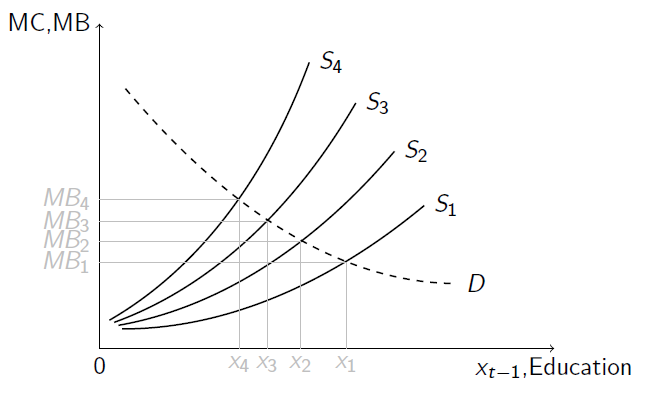
\includegraphics[width = 0.45 \textwidth]{egal.PNG}
Why the supply of education varies isn't important, it could be a mix of family, wealth, subsidies and luck.  In this case we can identify the common demand curve from a cross section of individuals, and we can identify individual marginal rates of return from looking at earnings at different levels of investment. We should expect that HC investments are more unequal the more unequal the distribution of (individual) supply curves is, and earnings will depend on investments and the returns to education. If the demand is completely elastic, we have that $earnings = k x^*$ where $k$ is the returns to \$ 1 invested in education. Since we normally take that demand is downwards sloping, as HC is embedded in the individual we should see that earnings were less unequally distributed than $x^*$. So to sum up
\begin{itemize}
\item More elastic demand $\rightarrow$ more unequal $x^*$ and earnings
\item More elastic supply curves $\rightarrow$ more unequal $x^*$ and earnings
\end{itemize}

\paragraph{The elite case} is the exact opposite. Here only individual demand varies, while supply is the same for everyone, so we have some variation of 'equal opportunities'. 
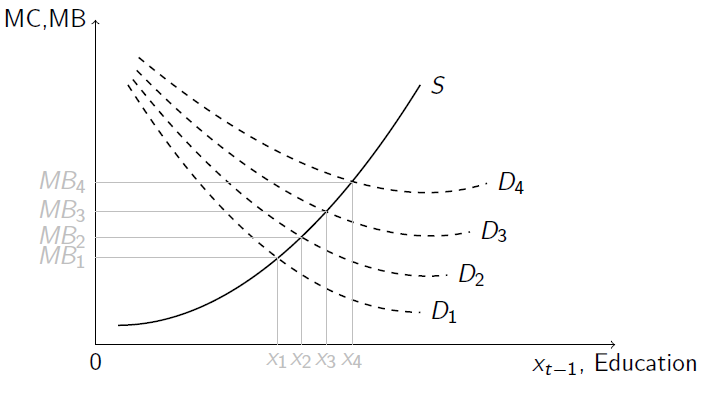
\includegraphics[width = 0.45 \textwidth]{elite.PNG}
The higher ones demand-curve, the more HC one produces with a given investment level. Here we can indirectly measure ability by looking at ones earnings given a constant $x$, and identify the common supply curve by a cross section. Unlike in the egalitarian case the individual marginal rates cannot be identified from earnings and investments. Similarly to the egalitarian case HC investments are more unequal the more unequal the demand curves are, but in the elite case earnings are more unequally distributed than $x^*$, assuming supply slopes upwards. 

\paragraph{Comparing the two cases} 
In the egalitarian case we see that the higher $x^*$, the lower the marginal benefit, while in the elite case it's exactly opposite. Empirically both cases have been found. 
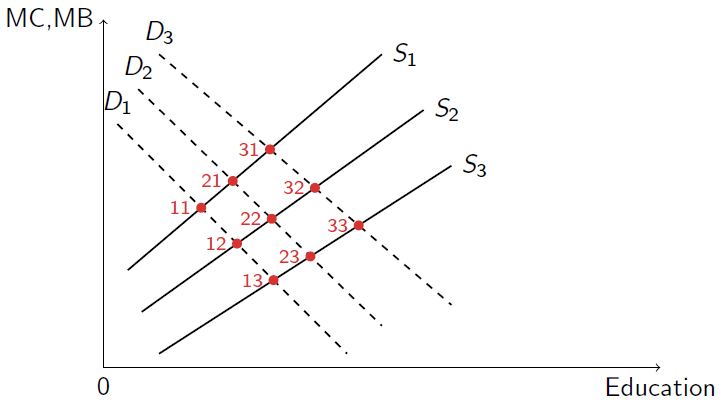
\includegraphics[width = 0.45 \textwidth]{comp.PNG}
Furthermore the egalitarian case has less inequality in earnings than in supply (as the demand curve compresses the distribution) while in the elite case income is more unequally distributed than $x^*$. Thus the egalitarian case needs to assume a relatively large variation in funding rates, while the elite case must assume relatively low variation in abilities, to explain the income spread. In the elite case standard assumptions show that a symmetric ability distribution can produce a varied and skewed income distribution.
\\ \\
It's entirely possible that supply and demand conditions are correlated, for example through family background (on the other hand targeted subsidies might alleviate such correlations).
\begin{itemize}
\item A positive correlation - would increase inequality in investments $x^*$ and in earnings (this would increase investments for those who already invest a lot, and decrease investments of those with low investments to begin with). Thereby increases skewness. We can think of this as a straightforward effect where high demand brings with it high supply.
\item A negative correlation - where higher demand lead to lower supply. If we observe individuals choosing the same $x^*$ regardless of differences in MC, this shows their curves are negatively correlated. 
\end{itemize}

\section{Part 2 - Evidence on credit constraints and inequality}
\subsection{Lecture 5 - Micro evidence on credit constraints}
It's a persistent and robust finding that there's a gap of educational attainment and college enrollment by family background and cognitive abilities, so that better-background children get significantly more education. This is mainly explained with either credit constraints and/or consumption value theory. Ellwood \& Kane(2000) use micro data to control for ability, but still find large differences in attainment by income, they take this as evidence of borrowing constraints. On the other hand Cameron \& Taber (2004) use as foundation that heterogeneity in rates of return would imply different borrowing rates, so they use IV to test for heterogeneity. They find no results and conclude that borrowing constraints are not important. 
\\ \\
\paragraph{Keane \& Wolpin (2001)} find that students are very tightly constrained, but that borrowing constraints have little influence on completion, so increasing loans would only lower labor supply and increase consumption. 
\\ \\
\paragraph{Carneiro \& Heckman (2002)} use ability at age 17 as control, and find no evidence of borrowing constraints. They hypothesize that because family income is correlated over time, borrowing constraints are not especially binding at college age, instead a lifetime of budget constrained decisions add up and leaves a trace in abilities. Thus borrowing constraints are already binding before college.   
This means government programs should shift focus from providing funds, to improving college preparedness for children in low income families. 
\\ \\
\paragraph{Belley \& Lochner (2007)} contrast the '79 and '97 version of the National longitudinal survey of youth (NLSY), combined with army tests of skills and knowledge. The two cohorts vary slightly, the newer cohort is more educated, less white and has a wider income distribution. They find that ability determines completion rates, but that these also vary substantially with family income. Especially for the poor youth, income has become more important between '79 and '97. They also show that the rise in high school completion rates are distributed evenly across all income levels, but that the rise in low-ability students come entirely from high income families. They find significantly higher attainment in children with educated mothers, intact 2-parent families and minority background. 
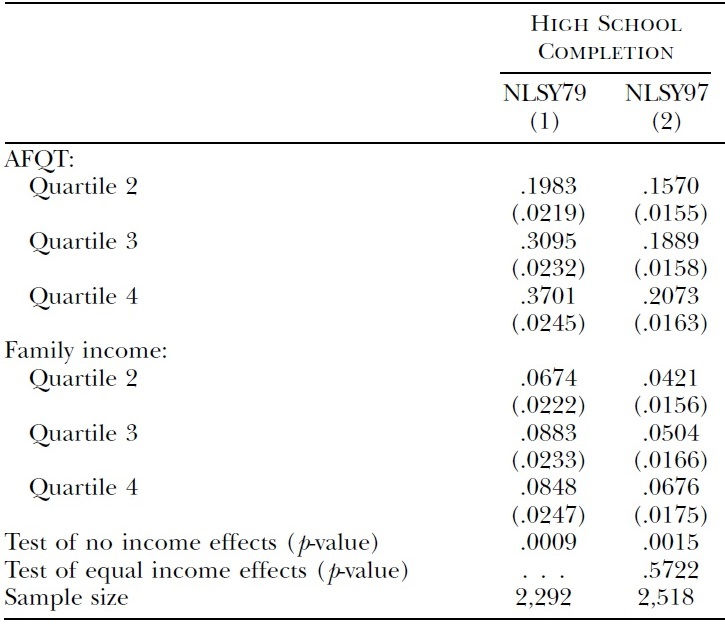
\includegraphics[width = 0.45 \textwidth]{belleyL.jpg}
From the table it's evident that "ability" (AFQT is an army IQ test) is more important at the bottom, while family income has a modest effect. 
The authors carry out a number of robustness checks, including family income per capita, other ability measures, economic conditions (business cycles) and net family wealth. 
\\ \\ 
A competing explanation to the credit-constraint hypothesis is that of \textbf{consumption value}. We ask if education is a good or a bad, that is if 
\begin{itemize}
\item[A)] Education is a good - high income families purchase more of it
\item[B)] Education is a bad - there are psychic costs to education, people are willing to pay to avoid it, so high income families pay to avoid it
\end{itemize}
Let tuition be a function of wealth $W$, and let returns to education be increasing in ability $A$. Finally include a consumption value of college $\xi$, so that college attendance happens if 
\begin{align*}
v_1(W,A)+ \xi \geq v_0(W,A)
\end{align*}
where $v_1$ is the valuation of going to college, and $v_0$ is the valuation of abstaining. Those at the margin of attending college then have
\begin{align*}
\xi = v_0(W,A) - v_1(W,A)
\end{align*}
and since the financial returns to college are positive we must have $v_1-v_0>0$ so $\xi<0$ which shows that there is a psychic cost of college. Then note that high-ability students will generally have more negative $v_0-v_1$ so they have a great distaste for college. If they're from higher income families, they can then pay to avoid college, which should give us a negative income-attendance relationship for the highly skilled. Oppositely if someone has a very low $A$, the value of college may be negative, giving them a positive $\epsilon$ - for them education is a good, and high income families will purchase it for their low ability children. This gives us the prediction that income/attendance should be decreasing for high ability individuals, while increasing for low ability individuals (unless tuitions depend on income $T=T(W)$ in which case the low ability case is ambiguous). This however contradicts data, so we will have to include credit constraints.
\\ \\
Assume a borrowing limit of $\bar{D}$, so that if $A>A^C(W, \bar{D})$ an individual is constrained, then high ability youths are constrained as returns are increasing in $A$. Thus high ability individuals would like to borrow more and smooth consumption against their future return. Therefore the value of college is increasing in the borrowing limit for those who are constrained. We should expect the following changes between the two cohorts:
\begin{itemize}
\item[1)] An increase in tuition levels will reduce $A^C$, meaning more are constrained. Those unconstrained are also discouraged, with the highest effect on low-ressource low ability individuals. This leads to a more positive resource-attendance relationship
\item[2)] Reduced borrowing opportunities decrease attendance for all. The effect is biggest on low income/high ability families, also giving a stronger resource-attendance relationship. This also extends the range of $A$ in which people are constrained, which extends the positive res-attend relationship to lower levels of $A$.
\item[3)] An increase in the college wage premium - increases attendance for all, but also means more are constrained, also meaning that previously unconstrained low $A$ types become constrained.
\end{itemize}
All 1)-3) imply a larger fraction of the population will be constrained, but 2) imply reduced attendance rates, which is not observed in the data. The high income students in the 97 cohort is more likely to attend 4 year college than their less endowed peers, while this is not true in the '79 cohort. This points towards college becoming less attractive for low income youth (rising tuition levels, worse borrowing opportunities) while high-income youth benefit by attending college and working at the same time. Of course the idea that this is caused by either 'college preparedness' or credit constraints is not certain - it could as well be network effects or imperfect information.

\subsection{Lecture 6 - Macro evidence for credit constraints}
It's a long standing hypothesis that growth shapes inequality, and empirically it's clear that income inequality is negatively related to growth. One explanation to this could be borrowing constraints limiting the access to education (although this is not at all certain, it could just as well be that inequality causes uprising, which in turn lowers growth). To understand if education might be the cause we propose that optimal schooling is given by some
\begin{align*}
S_{it}=g(\underbrace{A_{it}}_{(+)}, \underbrace{Y_{it-1}}_{(+)}, \underbrace{\beta_{t}}_{(+)}, \underbrace{s_{t-1}}_{(+?)})
\end{align*}
where most variables are as standard, $\beta$ is the returns to schooling. It should be noted that here $A$ is purely positive unlike in the Becker-Tomes model, where the combined effect of higher $A$ lowering marginal utility from parents consumption and increasing returns to investments, means it's difficult to tell what effect higher ability have. Taking that $A_{it}=h(A_{it-1})$ and $Y=f(A,S)$ which inverts to $A_{it-1}= f^{-1}(S_{it-1}, Y_{it-1})$ we have
\begin{align*}
S_{it}=g(\underbrace{h(f^{-1}(S_{it-1}, Y_{it-1})) }_{(+)}, \underbrace{Y_{it-1}}_{(+)}, \underbrace{\beta_{t}}_{(+)}, \underbrace{s_{t-1}}_{(+?)})
\end{align*}
By assuming this function to be log-linearizable we can then test 
\begin{align*}
s_{it} &= \alpha_0 + \alpha_1 s_{it-1} + \alpha_2 y_{it-1} + \alpha_3 y_{it-1} \\
& + \alpha_4 \beta_t + \alpha_5 s_{t-1}
\end{align*}
Here $\alpha_2>0$ would suggest ability inheritability and $\alpha_3>0$ that liquidity constraints are present, unfortunately they cannot be separated, so the only strong conclusion would be if they were both 0. Essentially what we have is 
\begin{itemize}
\item[$\Rightarrow$] if optimal demand for schooling is a function of ability, and this is inherited, we should have a positive correlation between schooling and income
\item[$\Rightarrow$] If liquidity constraints prevent the poor from attending college, we should have a positive correlation between schooling and income
\end{itemize}
So as stated our best option is to hope for a coefficient of 0. To work around this issue, we can consider a cross section of countries, and replace $y_{t-1}$ with the Gini index. In this case a negative relation between gini and enrollment rate would be present if poor families are actually credit constrained. Furthermore this should give us a positive relation between public expenditures and enrollment rates, as public expenditures would then loosen the credit constraints.
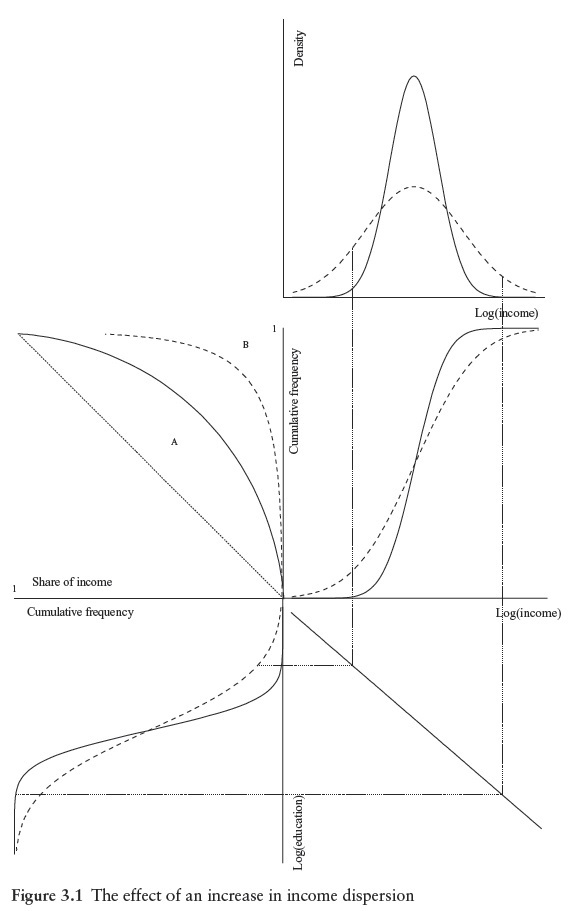
\includegraphics[width = 0.45 \textwidth]{dist.jpg}
The figure shows the relationship between income distribution and inequality - if income becomes more unequal (dashed line) this translates to more unequal educational attainment and thereby a more unequal Gini. Analysis in diagrams like this will show that increases in mean income, while maintaining the variance will not change inequality, and likewise by shifting the lower right line we can analyze the effect of increasing public expenditures.
\\ \\
Running regressions on the hypothesis shows little sign of relation in primary school, only variables like 'students per teacher' increases attainment. In secondary education there is some evidence of a negative correlation between gini and enrollment, especially for females. Here governments can mitigate the inequality effects by increasing spending. In higher education the effect is again low, and only present for males. 

Both secondary and higher education seems to be most influenced by the completion rate on the 1-below level of education. Checchi interprets these results as evidence for credit constraints and concludes that governments should boost spending on education. If his transition between individuals income and the income distribution is sound is however not clear. 

\subsection{Lecture 7 - Inequality and intergenerational persistence}
Say in a family the father has permanent income $Y_{fi}$ and the son $Y_{si}$, then the intergenerational earnings elasticity is defined as $\rho$ in
\begin{align*}
y_{si} = \alpha_0 + \rho y_{fi} + \epsilon_i
\end{align*}
where $x = \ln X$. We can interpret $\rho$ as how much the sons income will be above the mean, if the fathers income is $N$ above the mean. If the variance on the income of son and father is the same, we can further say that $\rho$ is the correlation between fathers and sons earnings. Here $y_f$ are long-term earnings, but these are rarely available in data - and might therefore be miscalculated. The temporary income is $y_{kit}=y_{ki}+ v_{ki}$ where $k\in\{f,s\}$, so we will have errors-in-variables biases in our estimate of $\rho$ given by
\begin{align*}
\underset{N \rightarrow \infty}{\text{plim}} \rho = \rho \cdot \frac{\sigma^2_{yfi}}{\sigma^2_{yfi}+ \sigma^2_v}<\rho
\end{align*}
To fix this we can use an average of the fathers earning $\bar{y}_{fi} = \frac{1}{T}\sum_{t=1}^T y_{fi}$ whereby we get

\begin{align*}
\underset{N \rightarrow \infty}{\text{plim}} \hat{\rho} = \rho \cdot \frac{\sigma^2_{yfi}}{\sigma^2_{yfi}+ \sigma^2_v/T}<\rho
\end{align*}
which shows that the inconsistency is then decreasing in $T$. The next problem is that wages have a clear life-cycle pattern, so $v_{fit}, v_{sit}$ are functions of age, therefore comparing an old fathers earnings, to those of a young son also underestimate the lifetime link. This can be handled by adding age controls to the regression.  

Next we need to devise of an instrument for the fathers earnings, here one proposed measure is the predicted earnings of the father, based on his educational level (these covary with his \textit{permanent} income). Only issue is if fathers education still covaries with sons earnings after controlling for the fathers permanent income - that is education doesn't fully strike out in income. In this case $\rho$ will be upwards biased. 

Similarly our measurements of the sons earnings are potentially misleading, if high-potential sons begin earning money later than others, but have a steeper wage growth, we might underestimate their permanent income which induces a downwards bias on $\rho$.

\subsubsection{Empirical evidence on $\rho$}
Early estimates of $\rho$ were around 0.20 (Becker \& Tomes, 1986) implying a very mobile society - later estimates have corrected for a number of measurement issues, implementing longer panels, older sons and more representative samples. Here estimates of $\rho$ are in the range of 0.30 to 0.50. Chetty et. al have later used tax data to find an estimate of 0.34, while Mazumder(2005,2016) claim tax data still have issues with young sons and short panels. His estimate is 0.60 or higher. 
\\ \\
The estimates on daughters are scarce, because of the lower labor market participation rate. Chadwick and Solon find an estimate of $\rho = 0.43$ for daughters, and 0.36 for daughters husbands, which they take as evidence for 'assortative mating'. Mazumda have also done work to show estimates are similar for sons and daughters in the US. 
\begin{center}
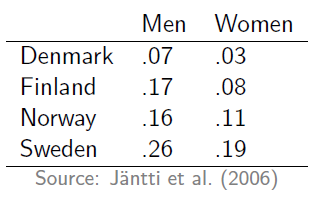
\includegraphics[width = 0.3\textwidth]{rho.PNG}
\end{center}
In the nordic countries estimates are lower, indicating a more mobile economy in terms of intergenerational mobility. It's conjectured and likely that these estimates are generally higher in developing countries. 
\\ \\
It's unclear if the differences in estimates are due to measurement errors. On one hand the nordic countries are more equal than the US and have lower estimates, but at the same time Canada has about the same $\rho$ as the nordic countries, but is approximately as unequal as the US. 
\\ \\
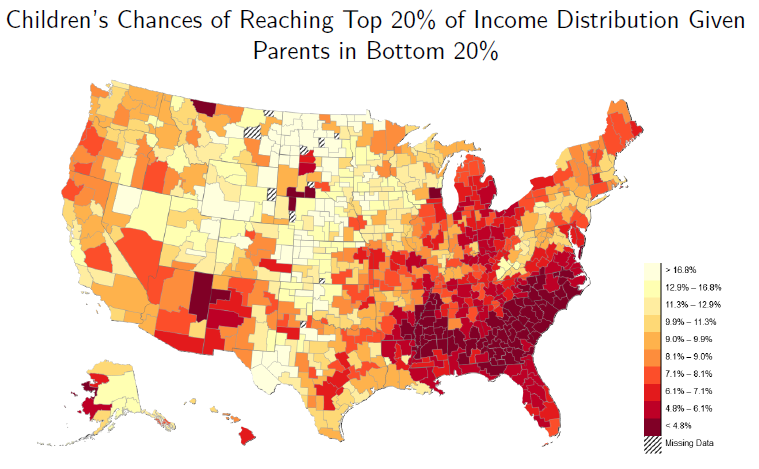
\includegraphics[width = 0.5\textwidth]{map.PNG}

\subsubsection{causes for persistence in earnings across generations}
One way to examine the origins of intergenerational persistence is to use adoptions as natural experiments. There is partially independent variation in prebirth $(b)$ and postbirth $(a)$ environments, so Björklund et al. use a sample of adoptees born in Sweden in 1962-1966, they then write the post-birth relation as 
\begin{align*}
y_{si}^a = \alpha_b y_{fi}^b + \alpha_a y_{fi}^a + \epsilon_i
\end{align*}
They then measure the characteristics of the father by years of schooling, earnings and likewise for mothers. They find total estimates of $\rho$ in the range of 0.24-0.34 on fathers characteristics, about equally distributed between $\alpha_a$ and $\alpha_b$ (estimates are slightly lower for mothers) so they conclude that pre-birth factors, as well as adoptive parents matter. Furthermore they find that biological mothers are more effective than adoptive mothers, whereas it's opposite for fathers. They also find strong interaction effects, that is having high $y_{fi}^a$ and $y_{fi}^b$ gives a stronger benefit.

Their results have been critiqued, for not taking into account that adoptees are not randomly assigned to adoptive families, instead disadvantaged children are placed in strong families. Also adoptees must be moved immediately at birth for their analysis to hold, and adoption itself might affect outcomes drastically due to adverse psychological effects. 

\paragraph{Restuccia and Urrutia (2004)} builds a model where individuals live 2 periods as children and 2 as adults. They calibrate the model on US data and find that most persistence in abilities is present already after early education, which amplifies the exogenous persistence. College on the other hand reduces persistence very slightly.

Most disparities in earnings are generated at the college level, but a large share is already explained by the innate differences. In their setting a lower college premium reduces the persistence in earnings, as the returns to education make rich parents dial back on  investments, while the poor who were previously unconstrained keep up investments. 

The authors can also do experiments in their setup, for example they allow a 1-time lump sum transfer of 30\% of total college tuition costs. Among the young parents 30\% increase their investments in early education, but spend only 14\% on the transfer while consuming the rest. Among the old parents even fewer change college decision.

By increasing public expenditure in early education with 20\% intergenerational persistence in earnings drop by 10\%, and persistence in education and consumption drops as well. The interpretation is that government expenditures work as partial substitutes for credit markets.

Doing the same experiment on public expenditures towards college leaves earnings persistence unchanged - only persistence in educational attainment drops. The issue is that the policy benefits children from poor backgrounds to late. Even though enrollment rates increase, the lack of ability from early childhood drives up dropout rates as well. 
\\ \\
Because ability is unobservable it's impossible to target funds at credit-constrained families, therefore governments should subsidize early education, where all income groups are affected. 

\section{Part 3 - Returns to education}
\subsection{Lecture 8 - Returns to education}
Imagine wanting to contrast two education levels, 0 or $s$, where earnings are respectively $W_t$ and $W_t^s$. Then the net-present-value of $s$ at age $t$ is the gain in wages, less direct costs $\gamma$ and opportunity costs $W_t$, that is 
\begin{align*}
NPV(s) &= \overbrace{\sum_{t=s+1}^T \left( \frac{W_t^s - W_t}{(1+\beta)^{t-1}} \right)}^{\text{gains}} \\
& -\underbrace{\sum_{t=1}^s \left( \frac{\gamma + W_t}{(1+\beta)^{t-1}} \right)}_{\text{costs}} 
\end{align*}
The internal rate of return (IRR) is defined as the discount rate $\beta = \rho$ so that $NPV(s) = 0$, i.e. where
\begin{align*} 
\sum_{t=1}^s \frac{\gamma + W_t}{(1+\beta)^{t-1}} = \sum_{t=s+1}^T \frac{W_t^s - W_t}{(1+\beta)^{t-1}}
\end{align*}
We can relate the IRR to a cross-section of wages through the Mincer assumptions, that is 
\begin{itemize}
\item Individuals doesn't work while in school
\item Foregone earnings are the only cost of schooling (or tuition + psychic costs are negligible)
\item Individuals work for the same number of years
\item Schooling and experience ($X_t$) have separate effects on earnings
\item log-earnings are linear in schooling
\end{itemize}
Then talking logs and rearranging gives an approximation of the previous equation
\begin{align*}
\ln W_{it}^s \cong \ln W_{i1} +s \cdot \rho + \beta_1 X_t + \beta_2 X_t^2 + \epsilon_t
\end{align*}
By adding a vector of observable characteristics $\mathbf{Z}\delta$ to account for individual differences in $W_{i1}$ we can control for background. Then taking population averages we can come up with an estimate for average $\rho$. This is exactly what Mincer did in 1974, he constructed the equation
\begin{align*}
\ln Y_i = \rho S_i + \beta_1 X_i + \beta_2 X_i^2 + \mathbf{Z}\beta_3 + \epsilon_i
\end{align*}
$\rho$ is known as the Mincer-coefficient as it can both be interpreted as the average percent-increase in earnings from an extra year of schooling, or by using the mincer assumptions, as the average IRR. In the US $\rho$ is in the range of 6-10\% and lower for developing countries.

In the 70's and 80's many countries experienced falling $\rho$'s but in Denmark returns increased significantly(from 2.5 to 4.5 pct). In recent years the rate has again been increasing in the US - seemingly at contrast with the large increase in college graduates, who should drive up supply. The Mincer equation is very often estimated in economics to provide a benchmark for further testing, but it is not without issues. First of by assuming one $\rho$ to hold over many different $s$, we've also implied that log-earnings are linear in schooling - this reduces to a hypothesis of no 'sheepskin effects', that is there is no extraordinary gain from finishing a degree, compared to not finishing the last year of the degree. 

Another relevant question is whether the mincer equation captures true causality, since things like parental background can influence both earnings and schooling. The most prominent of these omitted variables with potential to pollute estimates of $\rho$ is innate ability. To compensate for this studies have tried to include ability dummies such as IQ or test scores, but find that the effect of ability is small - only about 10\% of $\rho$ disappears after controlling for ability. Notably some tests of the importance of family background and ability's effect on earnings have been inconclusive, meaning some of the models studies in this course loose central parts of their explanands. 

\subsubsection{Twin studies}
Twins are the most identical individuals we can find in terms of background and genetics. Furthermore most families invest equally in their children, making them vary little on background characteristics. If we can find twins with different levels of education, they're therefore ideal to study, as we avoid many of the potential biases. Twin studies yield estimates of $\rho \in [6\%,12\%]$ in the US, and around 2-5 in UK/SWE. 

On danish data it's possible to compare mono- and dizygotic twins on registry data, and we can therefore decompose returns into observed- and unobserved ability. These findings suggest that unobservable ability account for a very little part of the increase in returns. Critics have pointed out that genotype $\neq$ phenotype and that even monozygotic twins can vary both genetically and in terms of upbringing - claiming otherwise makes it very hard to answer why twins differ in their choice of education in the first place.
\\ \\
Another class of research uses natural experiments, such as features of the schooling system or geographical differences to examine returns to education. A good example is 'increases in compulsory schooling laws' which force one year of students to complete an extra year of education, compared to their older peers. 

A subgroup of these use IV estimations to filter out endogeneity. When using instruments we should aske the following
\begin{itemize}
\item Does the instrument affect schooling and how?
\item Who is affected (who's at the margin affected by the instrument)?
\item Does the instrument affect earnings directly? (it shouldn't)
\end{itemize}
Importantly instruments can only uncover the effect of a change in policy in those whose decisions are altered by the new policy. Always- and never takers are not affected, so estimates will not reflect their 'true parameters'. We say instruments doesn't identify average effects, but only the effect on a subgroup which is affected. IV estimates tend to be in the range of 10-15\%, which is higher than the OLS estimates. This does not necessarily mean the true effects are greater - first of IV estimates tend to have larger variance, and secondly the instruments only affect subgroups, and it's likely that policy targets the subgroups that have the highest gains. 
Some natural experiments, like increased compulsory schooling years, are only effective for those who would otherwise quit school after minimum time, and they are likely to be poor-background low ability individuals. 

It's repeatedly been found that returns are higher for females, those who finish a degree (instead of finishing any other year) and academic educations.

\subsubsection{Evidence from school construction in Indonesia}
Duflo (2001) studies Indonesias INPRES program, which began in 1973. INPRES began major development of the schooling system, and constructed 61.000 new primary schools in regions with low enrollment rates. As a result enrollment rates for those aged 7-12 rose from 63\% in '73 to 83\% five years later. Duflo then constrasts those age 12-17 (control) and those age 2-6 (treatment) in 1974, to find the effect of the increased schooling. A diff-in-diff approach reveals a return to education of $27\%$.

\section{Part 4 - Signaling}
\subsection{Lecture 9 - signaling}
In the previous lectures we've assumed that education is productive, and that returns to schooling reflects differences in individuals productivity. Alternatively schooling might simply be a sorting mechanism which allows individuals to signal their innate abilities. This introduces issues of incomplete or asymmetric information. If firms cannot observe ability and are risk neutral, they will pay the average marginal product from the expected ability distribution. Mathematically assume there are two types of workers where $A_L < A_H$, where $\mathcal{P}(A=A_H)=n$. Workers marginal product is $f(A)$, and firms know the value of $A_L,A_H, n$ and the form of $f(\cdot)$. We then have
\begin{align*}
\bar{A} = nA_H + (1-n) A_L
\end{align*}
and 
\begin{align*}
\bar{W} = n \cdot f(A_H) +(1-n)f(A_L)
\end{align*}
If we assume a constant marginal product $f(A) = \phi A$ we get
\begin{align*}
\bar{W} = \phi \bar{A}
\end{align*}
But this in turn implies $\bar{W}<W(A_H)$ and $\bar{W}>A_L$, in other words high ability workers subsidize the low ability types until the wage differential is 0. The high ability workers might want to signal that they're high ability, in which case the necessary conditions are 
\begin{itemize}
\item[$N1$] Signaling costs decrease with increases in unknown ability
\item[$N2$] The wage schedule incentivizes signaling
\end{itemize}
To fulfill these, assume that individual preferences are given by
\begin{align*}
V_i = W(S_i)-\gamma(S_i,A_i)
\end{align*}
where wages and costs depend on the signal. We assume that the cost of schooling obey $\partial \gamma /\partial S>0$ and $\partial \gamma /\partial A<0$. Like there are two ability levels, we assume there are only two signals $S_L<S_H$. With this setup it's profitable to invest in the signal iff 
\begin{align*}
V(S_H,A_i)&>V(S_L,A_i) \\
W(S_H)-\gamma(S_H,A_i)&>W(S_L)-\gamma(S_L,A_i)
\end{align*}
A separating equilibrium then consists of a situation where all $A_H$ types choose the signal, while $A_L$ types doesn't, summarized in the condition
\begin{align*}
&\gamma(S_H,A_L)-\gamma(S_L,A_L) \geq W_H - W_L \\ 
&W_H-W_L > \gamma(S_H,A_H)- \gamma(S_L,A_L)
\end{align*}
so the optimal wage differential depends on the cost function $\gamma$, but regardless of the exact functional form we need the signal to be profitable for high ability types, while being costly to low ability types. If this is the case the right set of wages announced by the firm can cause self-sorting.
\\ \\
If education is purely a signal, this solution is not pareto efficient, as the cost incurred by high-ability types doesn't affect their productivity. Instead they're essentially wasted resources.

\subsubsection{Screening}
An alternative to the signaling hypothesis is that the workers can pay to be screened and thereby reveal their type. This screening costs $\gamma$ for everyone. In this setting a separating equilibrium emerges if the cost of screening is lower than $W_H-W_L$ no high-ability type will ever screen. If the screening costs are smaller than $W_h - \bar{W}$, that is 
\begin{align*}
\gamma < W_H - \bar{W}
\end{align*}
High ability workers will accept screening. In this case the firm can change $n$ for each observed high-ability worker. The firm has an advantage, in that it can change it's wage policy and just assume that anyone who haven't been screened are low-ability. Then the condition for a separating equilibrium becomes
\begin{align*}
\gamma < W_H - W_L
\end{align*}
which is significantly better for the firm as $\bar{W}>W_H-\gamma >W_L$ -but for the high ability workers, this is a reduction in wages compared to the old policy that they're forced to accept as $W_L$ is still worse than $W_H- \gamma$. So in the screening case, both the low types and the high types get a wage that's lower than $\bar{W}$ - thus separation is \textit{pareto inferior} to pooling.
\\ \\
This should also show us that firms might want to screen privately, thus being able to select high skill individuals, while only paying $\bar{W}$. If workers don't know their talents either, risk aversion will lead them to not being screened even if $\gamma = 0$.

\paragraph{We can distinct between sorting and HC} by looking at self employed. Typically they earn significantly less than those on regular jobs, suggesting that some signaling or screening is at play. We can also try to track students who skip or repeat a grade, to see if this information changes wages - results however point towards no effect and thus the HC hypotheses.
Oppositely the 'sheepskin effect' (a year of education is much more valuable if its the year you finish your degree) point towards signaling as the driving force. At the individual level this doesn't matter much, as education gives you a payoff regardless of the reason, but for society the signaling hypothesis would mean we spend huge sums that are essentially unproductive. 

\subsubsection{Training - who pays?}
Training on the job is not uncommon, but the question is who pays and who benefits from it. Generally OTJ training gives either job-specific competences or more general use-anywhere competences. If we have perfect use-anywhere training, the abilities gained will be as useful in the specific firm as in any other firm, increasing the outside option of employees who get the training. If the job market is competitive this means a worker will require the increase in marginal productivity from training in wages - and thus the firm doesn't gain anything (disregarding network effects etc). What happens instead is that workers know training increase their future income, so they are willing to carry the cost of training through their wages. This gives rise to a concave earnings function, where only older workers take the full benefit of their MP, while younger workers 'pay' for training through their wages. 
\\ \\
Specific training is different in that it only improves ones ability to do the exact job one is working in (or is only partially applicable to other jobs). For fully specific job training, the outside option of workers is completely independent of training, and thus the firm only have to pay the outside options $W$ and can reap the benefits of $MP-W$. But if workers leave the firm, they take the trained abilities with them, so the decision of training employees must depend on the turnover rate. This means trained employees will still get some of the increased MP, to retain them. On an industry level, this might cause slow or sticky labor market adjustments in industries with large specific-skill-components, as both firms and workers loose from separation. 



\section{Part 5 - Skill formation}
\subsection{Lecture 10 - skill formation over the life cycle}
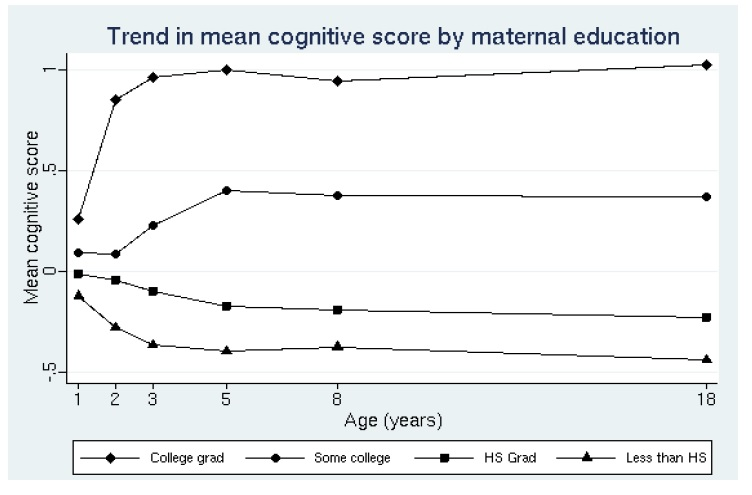
\includegraphics[width = 0.5\textwidth]{mateduc.jpg}
There's ample evidence that wealth or income increases with performance in the educational system, both when considering the worth of parents and children themselves. Heckman \& Moon study behavioral traits in relation to this fact, and find that among others, 'antisocial behavior' is decreasing in income quartile. Hart \& Risley find large differences in vocabulary of both parents and children across classes. In unison these observations show that gaps in abilities arise early and persist through childhood, indicating we should expect high returns to early investments compared to later. Furthermore if early investments are not followed up, the effect is lessened.

Credit constraints are effective, but how much depends largely on when they become effective. 

\paragraph{Cunha \& Heckman (2007)} use a simple model to describe the formation of skills over a life cycle, thereby uniting a broad body of evidence from various fields. In this they implicitly assume that inputs in the production of skills substitute perfectly between different stages of childhood. They seek to explain a world where there are
\begin{itemize}
\item Multiple stages of childhood - some of them more sensitive than others
\item abilities which are multiple in nature, and go together to create both cognitive and non-cognitive abilities
\item parental influences on children
\end{itemize}
The combination of parental influences and the multiple stages of childhood means credit constraints can work through three distinct channels
\begin{itemize}
\item[1)] The inability of a child to choose its parents 
\item[2)] The inability of parents to borrow against the future income of their child to finance investments in their child
\item[3)] The inability of parents to borrow against their own income to finance investments in their child
\end{itemize}
The model is set up as following: each agent posses a vector of abilities $\theta_t$ which range from cognitive (IQ) to non-cognitive (emotions) - these abilities are used with different weights in different tasks. Abilities are produced from family investments $I_t$. The technology of production of skill is given by
\begin{align*}
\theta_{t+1} = f_t(I_t, \theta_t, h)
\end{align*}
where $h$ are parental characteristics. We further assume that $f_t$ is neoclassical, that is strictly increasing, concave and at least $C^2$ in $I_t$. The main difference from previous production functions is therefore that parents now influence the productivity of HC investments. By recursive substitution of $\theta_t$ we then find
\begin{align*}
\theta_{t+1} = m_t(h, \theta_1, I_1, I_2, ..., I_t)
\end{align*}
This expression fits many of the requirements we wanted to have i.e.
\begin{itemize}
\item productivity of $h$ 
\item self productivity: $\frac{\partial f_t(I_t, \theta_t, h)}{\partial \theta_t}>0$ so $\theta_{kt}$ produces further $\theta_{kt+1}$, and cross effects so that $\theta_{kt}$ produces further $\theta_{jt+1}$. ($k$ is the vector index)
\item critical and sensitive periods
Sensitive and critical periods are is periods where investments matter especially much - we define a sensitive periods as a $t^*$ where
\begin{align*}
\frac{\partial f_{t^*}(.) }{\partial I_{t^*}} > \frac{\partial f_t(.) }{\partial I_t }, \quad t^* \neq t
\end{align*}
and a critical period as a period where 
\begin{align*}
&\frac{\partial f_t(.) }{\partial I_t } = 0 \text{ for } t \neq t^* \\
&\text{and } \frac{\partial f_{t^*}(.) }{\partial I_{t^*}}>0
\end{align*}
\item dynamic complementarity - which is that
\begin{align*}
\frac{\partial^2 f_t(.)}{\partial \theta_t \partial I_t'}>0
\end{align*}
thus we have \textit{static complementarity} between capabilities and investments within period $t$ (increasing abilities or investment increases the effect of one another). Between periods we have \textit{dynamic complementarity}, which is to say that the cross derivative between $I_t$ and $I_{t+s}$ is positive, so that raising $I_t$ raises $\theta_{t+1}$, which raises $\theta_{t+s}$ because of self productivity, so this raises $\partial f_{t+s}/\partial I_{t+s}$ because $\theta_{t+s}$ and $I_{t+s}$ are compliments.
\end{itemize}
Dynamic complementarity is essentially two distinct ideas, namely that 
\begin{itemize}
\item[1)] higher stock of abilities at age $t$ increase the productivity of investments at that age
\item[2)] Investments today raises the stock of skills in the future, and thereby raises the productivity of future investments.
\end{itemize}
It is the dynamic complementarity that explains why investments in more able individuals are more productive than for less able individuals. It also explains why returns are highest in the early years, and why it is important to invest not only in early years, but to continue reaping the benefits (continuing to invest) when agents get older. We can generalize the 2-period-childhood case by assuming investments act through a CES function, so
\begin{align*}
\theta_3 = m_2(h, \theta_1, [\gamma I_1^{\phi}+ (1- \gamma)I_2^{\phi} ]^{\frac{1}{\phi}} )
\end{align*}
Then for $\phi \leq 1$, the lower it is, the easier it gets to substitute investments in education in either of the two periods of childhood. Whether late 'rescue' of lacking early investments will work depends on the elasticity of substitution, a low substitutability would imply that late investments are most effective for those who also had high early investments - oppositely late investment will not help much for those who were already disadvantaged. This contradicts the 1-period-childhood model where diminishing returns makes investments in low-ability children more productive. 

The dynamic complementarity also imply that while there is an equity-efficiency tradeoff at later stages, it's not present for investments in early childhood.
\\ \\
That investments are more effective in the early stages of life is also empirically valid; returns to teenagers education are lower for the disadvantaged and less able individuals, and the later remediation is given, the less effective it is. Of course there's still evidence of resilience and partial recovery. It has been found that the most effective interventions target noncognitive abilities, socioemotional- and character skills trough mentoring and guidance. 
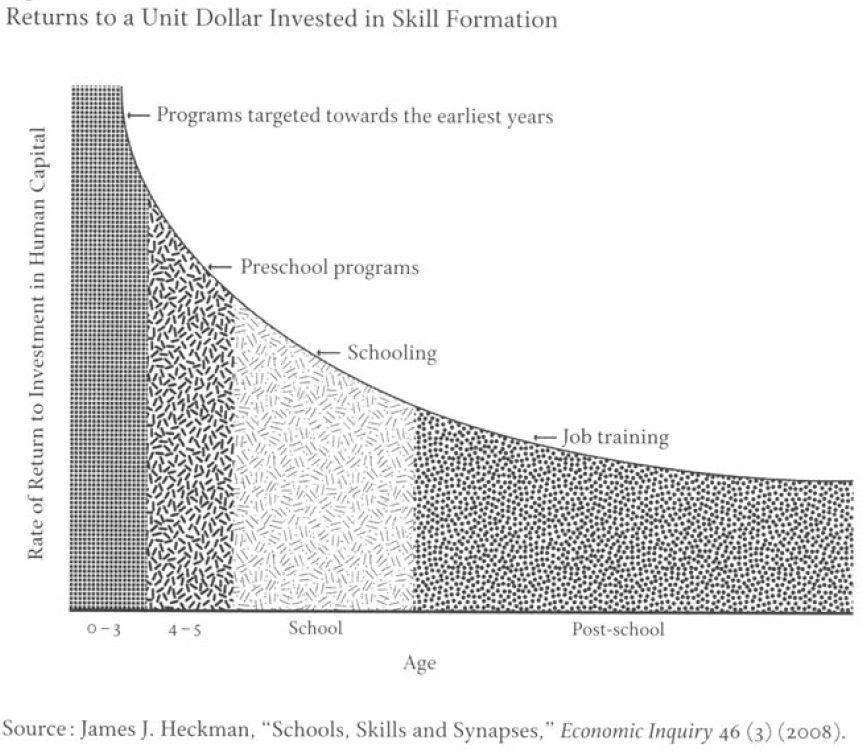
\includegraphics[width = 0.5 \textwidth]{returns.jpg}

\subsubsection{The Perry preschool project}
The Perry project is one of a small handful of controlled interventions in school policy, constructed to study the returns to early investments. Like the other studies the Perry project is small, and therefore potentially trades external validity for internal ditto. The program targeted low income black children from Michigan with an IQ below 85 at age 3. The program then consisted of 2.5 hours of 'active learning' for 5 days a week. After two full year the program stops, but subjects were followed until age 40. 

The researchers found strong effect of the treatment for both boys (graph below) and girls, varying in patterns by age. The program seems to have given a lifetime rate of return in the range of 7-10\% by comparing the costs of the program to estimates of the increases in lifetime wealth for the treatment group along with decreases in factors like crime etc. 
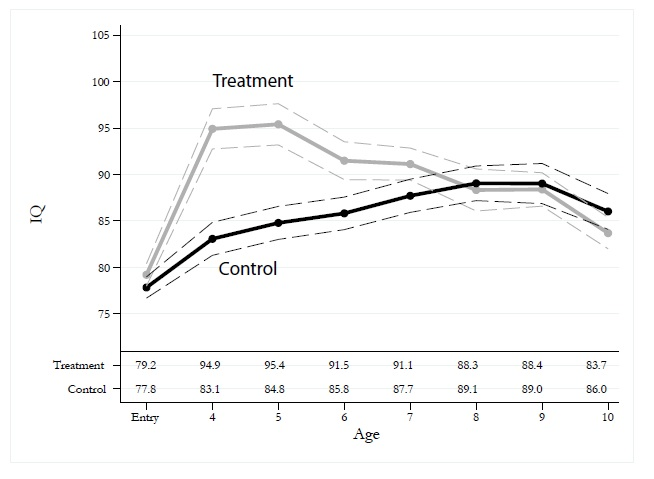
\includegraphics[width = 0.5\textwidth]{iq.jpg}
The program had positive effects on externalizing behavior and academic motivation for both boys and girls, 


\paragraph{Heckman et al. (2010)} Found further that female subjects of the program were held back in school less often (reducing costs), and attended more college classes (increasing costs). Those who did stay longer in school did however have an increased chance of getting a diploma, thus neutralizing the economic burden. They find no effects for males. 

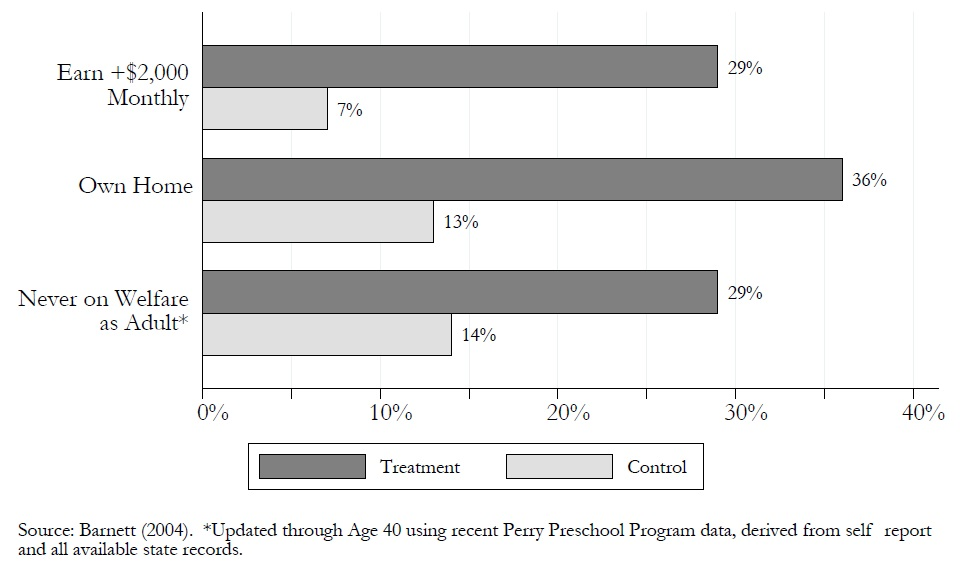
\includegraphics[width = 0.5\textwidth]{perry2.jpg}
Males in the treatment group also did substantially better than their control counter parts, in staying out of crime, indicating that the highest returns to the Perry preschool project stems from 1) higher earnings, resulting in higher taxes and 2) lower crime rates (crime is quite expensive).
\\ \\
In a number of studies like the Perry project the main channel for influence is through the parent-child relations, namely trying to give parents information, change their preferences and show interest in their childrens curiosity. This seems to have worked as both parents of boys and girls give greater weight to the importance of parenting after the end of the program.

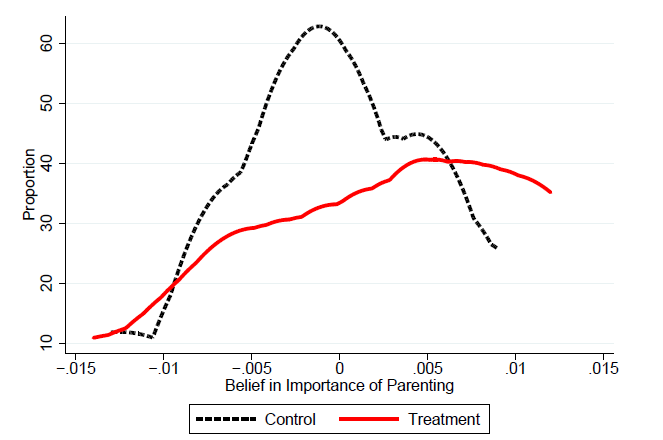
\includegraphics[width = 0.5 \textwidth]{perry1.PNG}\footnote{Parents belief in importance of parenting (female children)}

\subsubsection{Early childhood interventions - rationale}
It can be argued that governments should provide early childcare for three main reasons: 1) it has positive externalities, 2) credit markets seem to fail in providing it and 3) equity and redistribution concerns. Early childhood intervention brings both cognitive and non-cognitive benefits to children, and in turn society - but how it's implemented differs from place to place. Goals vary from the strictly cognitive to more environmental concerns (like nutrition) and intensity and setting varies as well. 

The cognitive benefits are shown to be present, but will in many case disappear when the children enters school depending on the quality of the programs. Furthermore children from low-income homes tend to benefit more. Medium- and long run programs have longer lasting effects on grades and educational attainment. Also the mothers(/parents) are from a governmental perspective better of with good early child care, as it allows them to reenter the labor market earlier. As there are large signs of intergenerational persistence, such programs can even help entire families out of poverty in the course of a few generations, although it's hard to test with the available data periods.

\section{Part 6 - Production of Schooling}
\subsection{Lecture 11 - The production of skills in school}
How schools operate is not unimportant to the skillset their students achieve. The evidence broadly categorizes as follows 
\begin{itemize}
\item Increased spending on schools
\begin{itemize}
\item Mixed evidence for financial inputs, but instruction time appears important, maybe also class size
\end{itemize}
\item Selecting teachers
\begin{itemize}
\item There's evidence of teacher effects, from adding more teachers ('teacher value added')
\end{itemize}
\item Selecting students
\begin{itemize}
\item There might be peer effects from the average quality of students - possibly indicating that sorting is a good idea. 
\end{itemize}
\item Expectations or 'educational values'
\end{itemize}
\paragraph{Resource effectiveness and class size} financial inputs can be used to decrease class sizes, or hire more teachers (somewhat identical?) 
\epigraph{Many of the 20 leading economic performers in the OECD doubled or tripled their education spending in real terms between 1970 and 1994, yet outcomes in many countries stagnated or went backwards. Educational performance varies widely even among countries that spend similar amounts per pupil. Andreas Schleicher, head of analysis at PISA, thinks that only about 10\% of the variation in pupil performance has anything to do with money.}{\textit{The Economist}}
We can generally measure resources either by classroom, e.g. teacher education and class sizes or by aggregate measures like spendings per student or teacher salaries. Empirically it's challenging to separate out the causal effects, as students are non-randomly sorted into schools by their parents, and initial characteristics are thereby correlated among pupils. 
\\ \\
Class size effects are notoriously affected by endogeneity from family background, so we need more sophisticated methods to uncover causal effects (think randomization, natural experiments and high-frequent data to control for background). 

\paragraph{Krueger (1999)} randomly assigned students to different class sizes in grade 1-4, and in all grades he find that small classes increase performance. Later in 2001 Krueger \& Whitmore added information on the childrens entrance exams, and found that children from smaller classes were more likely to apply for college, especially among minorities. The actual test scores were small however. Experimentally they had issues with parents who's kids were assigned to large classes, opting out of the experiment. 

\paragraph{Hoxby (2000)} uses variation in birth cohort sizes and local regulation, to study if class sizes matters, and find no significant effects. 

\paragraph{Angrist \& Lavy (1999)} utilize an old israeli rule that set a maximum size of 40 students per class, and dictate that classes reaching student numbers above this level shall be cut in half. They don't account for parental choice of residence, and have low variation, but do find an effect of smaller classes in grades 4 and 5.

\paragraph{Woessmann \& West (2006)} use an international test of math and science and school fixed effects to estimate the effects of class size. To do so they compare 2 grades within the same school and control for school fixed effects, grades and background characteristics. They conclude no general effects from class size, but suffers from weak instruments in some countries. In France and Iceland they do have an effect on math classes, and in Greece and Spain on science classes. This might not reflect what's actually happening - both GR and IS have below average overall attainment and pay low teachers salaries, so it might just be that low-paid teachers are not competent to handle large classes. 
\\ \\
To sum up these studies differ in whether they look at the level-effects or in 'value added' from small classes, it's also not clear why some countries have effects while others doesn't. 

\subsubsection{Evidence for resource effectiveness}
\paragraph{Cortez et al.(2015)} have carried out a randomized experiment where they give low skilled student double algebra training and train them in verbal presentations. They find large test score gains, and even larger gains in terms of college enrollment rates. Of course their research face challenges in practical applications, as we would expect decreasing returns quite fast for such programs, especially for better able children. 

\paragraph{Lavy (2015)} use PISA scores and country level variations in instruction time on different subjects. He finds moderate effects, with one hour of teaching increasing the test score with only 0.06 standard deviations. Effects are larger for girls and immigrants and low scoring students. This shows instructional time can have inequality reducing effects. 

\paragraph{Angrist et al. (2010)} use the charter school program KIPP (students get a paycheck for conforming to a behavioral code) and lottery admissions into charter schools to investigate the effect of KIPP. They find increases in testscores for participation in KIPP.

\paragraph{Dobbie \& Fryer (2013)} use the fact that oversubscribed charter schools in NYC must admit students through a lottery. They also use regression techniques to control for observed difference between students at different types of schools. They find that traditional measures like class size, per-pupil expenditure and teacher training doesn't affect school effectiveness. From qualitative research they identify five working policies
\begin{itemize}
\item Frequent teacher feedback
\item Use of data to guide instruction
\item High dosage tutoring
\item Increased instructional time
\item (High expectations)
\end{itemize}
These five traits seem to explain about 45\% of the variation in school effectiveness. This suggests that many schools are operating within the production possibility frontier - Hoxby, 2000 have some evidence that increasing competition between schools alleviate this problem. 

\subsubsection{Classes and peer effects}
Schools can in many cases select their students, and almost always the class compositions - this allows them to use peer effects to their advantage.

\paragraph{Jackson (2010)} use rule-based student assignment in Trinidad and Tobago to investigate peer effects. He finds that being with high ability peers increases later performance, and that these peer effects are twice as large for girls. When testing for non-linearity (that is peers are only important at the top) results are inconclusive. 
\\ \\
Whether we can use sorting to outperform ordinary mixed classrooms depends on the linearity of peer effects. If we have linearity in the effects, moving a good student from his high-ability peers will reduce peer effects in the high class with $\Delta$, exactly the same amount as will be gained in the low-ability class. 

\paragraph{Carell, Fullerton and West (2009)} use the fact that people are randomly assigned to a group in the US Air Force Academy. They find significant individual increases in academic performance with the average SAT score of the group and nonlinear effects. According to them, low ability types benefit the most from being with high ability peers, but they also find that middle ability types benefit from being separated from their low-ability peers. 

On that basis they create an optimal sorting mechanism for designing peer groups, with the goal of maximizing the grades of the lowest ability students. This mechanism assigns low-A types to groups with high-A's also present, while the middle-A types are placed in their own groups. They then run an experiment where half of the new students are subject to the optimal mechanism, while the other half is randomly assigned to a group.

Contrary to expected they find a negative and significant effect of the treatment. Their explanation is that the treatment groups are more extreme in their composition. Specifically the low-A types loose so much in grades they outweigh the slight gain for middle-type groups. The high-type peers are unaffected by the treatment. 

\epigraph{Our results suggest that using reduced-form estimates to make out-of-sample policy predictions can lead to unanticipated outcomes.}{Carell, Fullerton and West }

\subsubsection{Teacher effects}
Identifying teachers with high 'teacher-value-added'(TVA) is of interest as it could identify best practices, as well as allow schools to award good teachers. 

\paragraph{Chetty, Friedman \& Rockoff (2014a, 2014)} gather data on 2.5 mio. students over 20 years, and control for background with the assumption that previous test scores capture all relevant noise. They find an association between TVA and student test scores, and that teacher quality varies much more within schools than between them. On average they find that better students have slightly better teachers. 

In the longer run high TVA increases students labor market outcomes, as students with high TVA teachers more often attend college, earn more, save more for retirement etc. Summing the returns for an entire class, an average teacher can earn his students \$ 1.4 mio compared to a bottom level teacher over their lifetime. 

\paragraph{Jackson (2016)} look at TVA on multiple outcomes and finds that high TVA affect non-cognitive outcomes like no. suspensions and absence, on-time grade progression and course grades. Then he shows that these parameters predict graduation and college attendance independently of test scores. His conclusion is that by focusing only on test scores, we miss important 'good teacher' effects. 


\section{Part 7 - Non private benefits of education}
\subsection{Lecture 12 - Education and crime}
There's a strong negative correlation between education and crime, in 1993 for example, 2/3's of incarcerated men in the US had not graduated high school. in the NLSY survey, 34\% of the lowest educated report income from crime, whereas it's only 17\% of those with high education. Grogger (1998) however finds that this link is not one of educ-crime, but rather income-crime. 

Crime like any other business has expected costs and benefits - but to understand it's link to education it's important to understand if crime is a career choice like any other, or functions as a last resort. I.e do youth drop out of school to sell drugs, or do they sell drugs because they dropped out of school. 

Wages determine the opportunity cost of crime, current wage losses are incurred to plan and commit crime, while future wages are lost because of incarceration and potential lost earnings potential. Therefore if education has a wage return, it influences the opportunity cost of crime. Education of course can also increase the returns to crimes like fraud and financial crimes, so naturally agents balance their increase in opportunity cost with the potentially increased returns. 

We might also hypothesize that education socialize students to not commit crime, and teaches patience (increases cost of expected punishment) and alters risk preferences. 

\paragraph{Lochner (2004)} Say that since learning occurs throughout life, the opportunity cost of crime should generally increase with age, as well as educational attainment. So for 'low-skill crimes' we would expect a negative correlation with both age and education. He models a situation where agent dynamically choose to 1) work, 2) invest in HC or 3) commit crime. They're endowed with initial skills $H_0$, learning ability $A$ and crime ability $\theta$ - they develop through $T$ periods. HC is accumulated by
\begin{align*}
H_{t+1} = H_t + f(I_t, H_t, A)
\end{align*}
where $I_t$ is time invested in education. It takes $k_t$ time to plan and commit crime, so the time available for work is 
\begin{align*}
1-I_t - k_t
\end{align*}
Resulting in at total wage from work of 
\begin{align*}
w_t H_t (1- I_t - k_t) 
\end{align*}
The returns to crime are given by $N(k_t, H_t, \theta)$ additionally engaging in crime means you run the risk of getting caught with $P(k_t)$, and once caught criminals pay fines $F$ and spend time in jail for $J$ years, where one can only consume $\underline{c}$, loose skills at a rate of $\delta$ and has a value function of $\Omega_t(H_t)$. Lochner then construct FOC's for the utility maximization problem and finds that 
\begin{itemize}
\item $H_t$ has a higher marginal payoff for those who avoid incarceration
\item Crime discourages contemporary investments in HC
\end{itemize}
For crime the FOC tells us that $H_t$ discourages crime as it raise direct and indirect costs, but it may also raise crime through $\partial N / \partial k$, so ultimately the investment decision will depend on future work and crime decisions.
\\ \\
We can study the effect of the levels of initial endowments by looking at unskilled crime, which doesn't improve in payoff with ability. Then 
\begin{itemize}
\item[$A$] \textit{learning ability}: high ability individuals will invest more, so they prefer spending time on education rather than crime in the early periods. Later on their opportunity costs have increased, so they commit less crime here as well.
\item[$H_0$] \textit{initial human capital}: Differences in skill persist over time, so high $H_0$ types will commit less crime, but if they invest in education or just work is unclear.
\item[$\theta$] \textit{Criminal ability}: high types will commit more crime, they thereby spend less time in school enforcing their future crime rate.
\end{itemize}
We can also analyze increases in graduate wages - they of course increase opportunity costs, but also increase the number of graduates, so all in all they decrease crime rates through two channels. Peculiarly those with high criminal potential will commit \textit{less} youth crime, because like the high ability types, they have a high opportunity cost of future imprisonment. 

\paragraph{Empirical evidence - Lochner (2004)} testing the hypotheses of Lochner has two main issues, namely that many of them are possibly spurious correlations, and might in fact be reversely caused. On top of this comes various concerns of omitted variables, for example that of peer effects. It might both be that those who drop out of school are negatively affected by peers to commit more crime, or that those in a 'gang' (aka bad peers) are encouraged to drop out of school. Even if we control for family background, networks effects etc. we might still have issues with unobserved individual characteristics such as patience, and local variations in spending on police and schools can possibly bias results. 

On top of all this comes the fact that measuring crime is difficult in itself - data on incarcerations or arrests, incorporate elements of the effects of education themselves as uncaught criminals/unreported crimes wont be represented. So to sum up Lochners ideas, schooling affect crime mainly because
\begin{itemize}
\item Schooling raises the opportunity cost of crime
\item Crime has direct financial and/or psychic rewards
\item Schooling alters preferences for risk and patience
\item schooling affects social networks and peers
\item schooling keeps youth busy - it incapacitates potential criminals
\end{itemize}
But many of these bullets are difficult to test and might suffer from reverse causality to a high degree. 

\paragraph{Lochner \& Moretti (2004)} Present IV estimates that use state variations in compulsory schooling laws over time. This eliminates factors like patience etc, and gives the causal affect of schooling on crime, assuming that changes in compulsory schooling laws are not related to the underlying propensity to commit crimes. They find that 1 year of schooling reduce the chance of imprisonment by 0,1 percentage points for whites and 0,4 for blacks compared to (0.83\%, 3,6\%) for dropouts. Their results are very similar to OLS estimates and show little effect beyond high school completion. 

On the state level an increase in the average education of 1 year reduces arrest levels by 11\%, with some subgroups like assault dropping over 30\%.
\\ \\
Empirically they still face the issue of measuring outcomes (arrests ect.) instead of crime itself, which can bias results if education influence the likelihood of getting caught. They therefore use self-reported crime from the NLSY. For whites education significantly reduce self-reported crime, while the data for uneducated blacks suffer from severe underreporting. Their results are robust to a large number of family background and ability measures.
\\ \\
From these results one might suggest to policy makers that crimes are extremely costly, both to victims and due to the incarcerations costs and justice systems. Lochner and Moretti calculate the returns to increasing education for 4 types of violent and property crimes. They find that a 1\% increase in the high school graduation rate would save the US economy almost \$ 2 billion - about \$1600 - \$ 2900 per male graduate. Hereof 14- 26\% would be in the form of increased private earnings.  


\subsection{Lecture 13 - Education and Health}
\paragraph{Lleras \& Muney(2005)} Like with crime, there are strong and significant correlations between education and health regardless of what measure is used. These figures far outweigh the similar numbers for the effect of health care spending on health, suggesting education might be a good place to start if trying to improve longevity. This correlation lasts when controlling for socio-economic factors. There are three main theories of why education could improve health
\begin{itemize}
\item education makes people better decision makers, or give them better information
\item poor health results in little education
\item there's a third variable at play
\end{itemize}
With data from three censuses each a decade apart researchers estimate the death rate of age groups by comparing how many remain throughout the three census rounds. This is not a very precise method, and they even end up with negative death rates for some age groups. With these data and changes to laws regarding compulsory schooling and child labor, we have the setup for a quasi-natural experiment. With a regression discontinuity design we can then estimate the effect of changing laws on education. Furthermore the researchers group the states by the number of people who were affected by the changes (i.e. many were effected if educational levels were generally low).

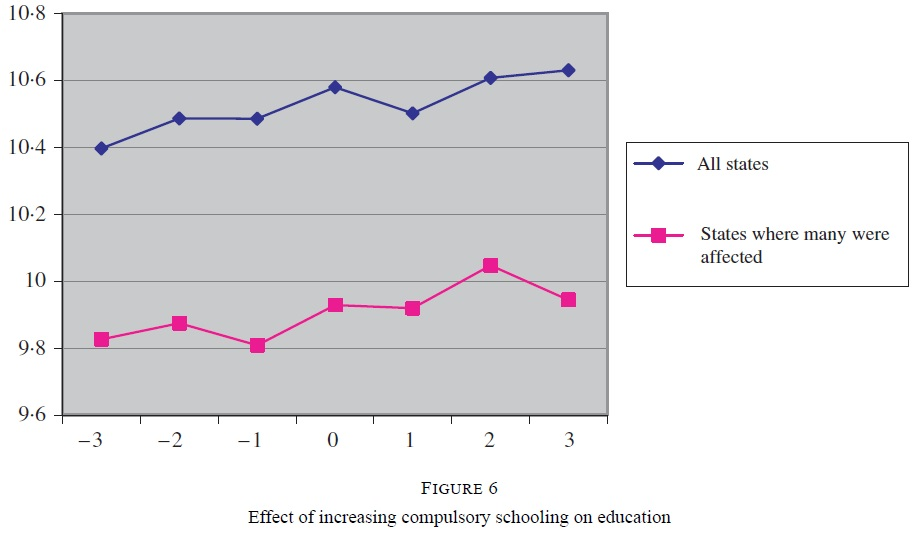
\includegraphics[width = 0.4 \textwidth]{compsch.jpg}

Across all measures the researchers find that increasing educational attainment decreases mortality with IV estimates, results are also significant with OLS, but generally parameters are smaller. This can be taken as evidence that the relationship between education and health is concave. In that case IV estimates, which only pick up the effect of those on the margin (low educ types) would be larger than the OLS estimates, which average the effect over the entire population. The no. years of compulsory schooling is also highly significant. In summary they find that 1 extra year of compulsory schooling decreases mortality by 3\%. 
\\ \\
Similar studies have been carried out in France and the UK, both resulting in insignificant results from education on mortality. 

\subsubsection{Why might education improve health?}
First of education might provide individuals with better reasoning skills, so treatments are more likely to be used properly by the recipients. For example diabetes patients generally comply better with the treatment). Additionally education might make people better at getting help, and process health information.

\paragraph{Grossman (1979,2000)} build a dynamic model of health investments as a form of investments in human capital. Here health effects the length of life, and thereby the return to education while education affects both health and labor market outcomes. One explanation of how this could work is by the mechanism where higher wage individuals get more health insurance which in turn increase their health - but evidence that health insurance increase lifetime is limited. This is partly due to an experiment by Rand (1982) where 4000 healthy uninsured were randomly assigned insurance. He found no evidence of changes in health, apart from for those already in the high risk group. Thus it's likely that investments in education give higher returns than in health directly. 
\\ \\
Education might also change behavioral traits, to increase focus on the consequences of unhealthy behavior, or simply make people better able to change behavior on the basis of information. The Perry preschool project observed increases in health of those who were subject to the treatment, and a decrease in risk factors like seatbelt use and smoking.

So even though it's hard to provide direct proof of a relationship, there's many indications that education might be a primary driver for health, and as Muenning, 2010 puts is "no consistent patterns can be detected between health and a third (omitted) variable". The most prevalent reasons of death are also clearly diseases that most often affect the low income parts of society.

\subsubsection{Other considerations}
One thing to consider is if it's family background that acts as a third variable, causing both educational attainment and health. These three variables all seem highly intertwined.

Over the last century both health and survival rates have improved enormously, and these trends will influence results if they're not handled in experimental designs. Considerations of this sort likely contribute to biases in the estimates obtained by many of the studies, and specifically can reduce the estimates of long run effects of education on health in regression-discontinuity designs.
\\ \\
Us data seems to show that education reduces problems with seeing, hearing and speaking, but not with walking, climbing stairs or lifting. In Europe results are generally weaker, and only partially support the hypothesis that education increases health. 



\subsection{Lecture 14 - Education and growth}
Returns to education are not only individual, as a highly educated workforce generate positive externalities on the country as a whole. All of the topics previously discussed, along with social cohesion and political insight might all benefit the GDP of a country. Three mechanisms through which this can operate are 
\begin{itemize}
\item[1)] Education increases HC
    \begin{itemize}
    \item This branch use variations of the Solow-model to study the aggregate effects of higher labor productivity
    \item There is (in the simplest of cases) transitional growth towards a higher steady state level of output.
    \end{itemize}
\item[2)] Education facilitates the diffusion and adaption of new technology required for economic development. 
    \begin{itemize}
    \item This should give permanently higher growth, is a hypothesis studied by (Nelson \& Phelps, 1966) and (Benhabib \& Spiegel, 1994)
    \end{itemize}
\item[3)] Education increases innovative capacity.
\begin{itemize}
\item This is mainly studied in the realm of endogenous growth theory.
\item education gives a sustained boost to the growth rate
\end{itemize}
\end{itemize}

\subsubsection{Macro approaches to returns to education}
In the macro literature there are two main approaches to education, the first incorporate education as an input in the production function, while the second can be thought of as a 'macro-Mincerian' approach, where the Mincer earnings function is estimated on macro data, i.e.
\begin{align*}
\ln Y = a + b S
\end{align*}
Some of the results in macro-education studies are that a 1 percentage point increase in primary school enrollment increases per capita GDP growth by 2.5 to 3\%, while a similar increase in KC stock increases per capita GDP growth by 12-17\%. Similar positive findings apply for years of schooling.

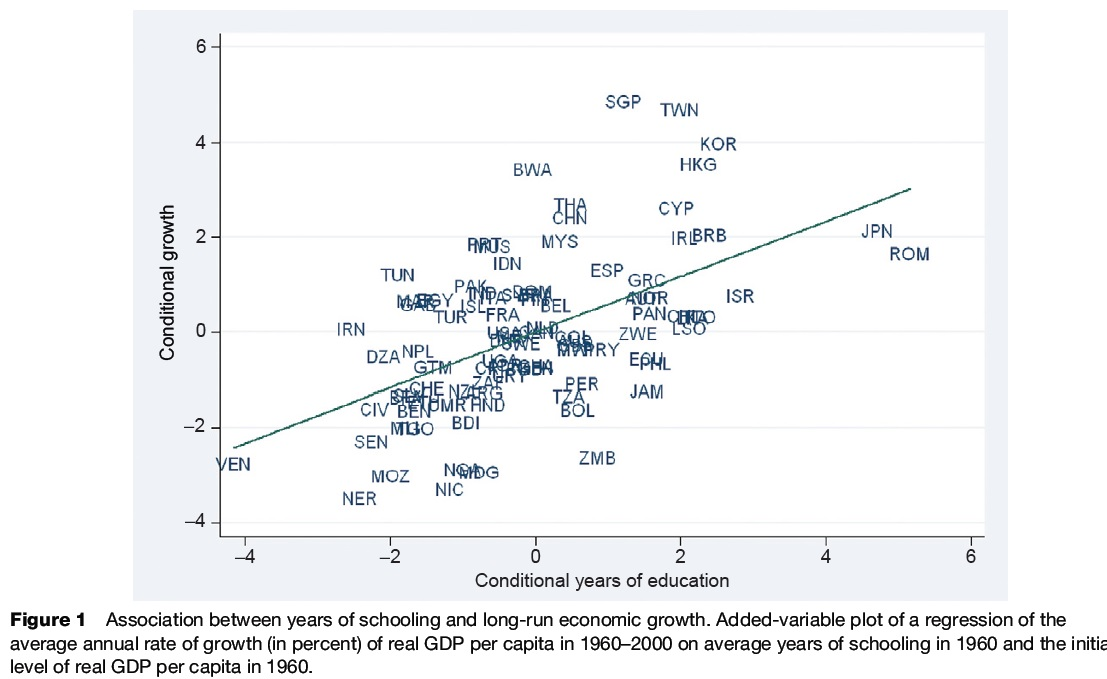
\includegraphics[width = 0.45 \textwidth]{plothanus.jpg}

Of course there are other explanations than schooling, first of all the possibility of reverse causality so that that GDP growth might cause increased schooling. Or it might be that the political regimes which promote growth also promote education (for example democracy). 
\\ \\
Criticism of the findings mainly focus on the quality of data, as they only register formal education, and are hard to compare across or even within countries. Many countries have large data gaps, which in some studies are extrapolated in, and often completely misses private schools. Lastly there are no good measures of educational quality, a potential source of omitted variable bias. 

\paragraph{Behrman \& Birdsall (1983)} say that quality is just as important as quantity, and on this basis contests the findings on macro level data. De Long \& Summers (1992) even find a negative relation between GDP and secondary school enrollment possibly because of "the large divergence between measured schooling and actual skills learned".

\paragraph{Hanushek \& Kimko (2000) and Hanushek \& Wössmann (2008, 2009/12)} study the effect of quality of schooling on growth. They find considerably larger gains from the quality of education than from the pure quantity, adding quality measures to the standard growth regression increases explained variance from 33\% to 73\% and makes years of schooling insignificant.
\\ \\
Cross country comparison requires assuming that all countries are on the same production frontier, but this is often not the case due to political or other social factors. To factor in these, they run the same regression while controlling for openness to trade and property rights, which still leave quality of education significant. There are however still other potential unobservables, for example "culture and discipline towards study and work". 

Another reason why cross country comparisons might fail is intra-country regional differences. In many developing countries the most highly educated are employed in the public sector, where they are less productive than their equally well educated peers in developed countries. 

Building on the lecture about crime, we might think that institutional factors determine if education gives the highest payoff in legitimate work, or in various forms of crime.
\section{Part 8 - technological change}
\subsection{Lecture 15 - SBTC}
\textit{*This lecture was all group activities about the SBTC*}

\subsection{Lecture 16 - Polarization and over education}
\paragraph{Autor \& Dorn (2013)} are interested in the polarization of the US labor market, into tow distinct groups of high- and low skilled workers. This has created a pronounced growth in wage inequality, so far explained by the SBTC hypothesis. The theory essentially says that modern technologies have favored highly educated workers, and have in some way been factor-augmenting to be complementary of high-skill worker traits. What the SBTC hypothesis so far haven't been able to explain is 
\begin{itemize}
\item A non monotone growth in the employment by skill level
\item non monotone wage changes by skill level
\end{itemize}

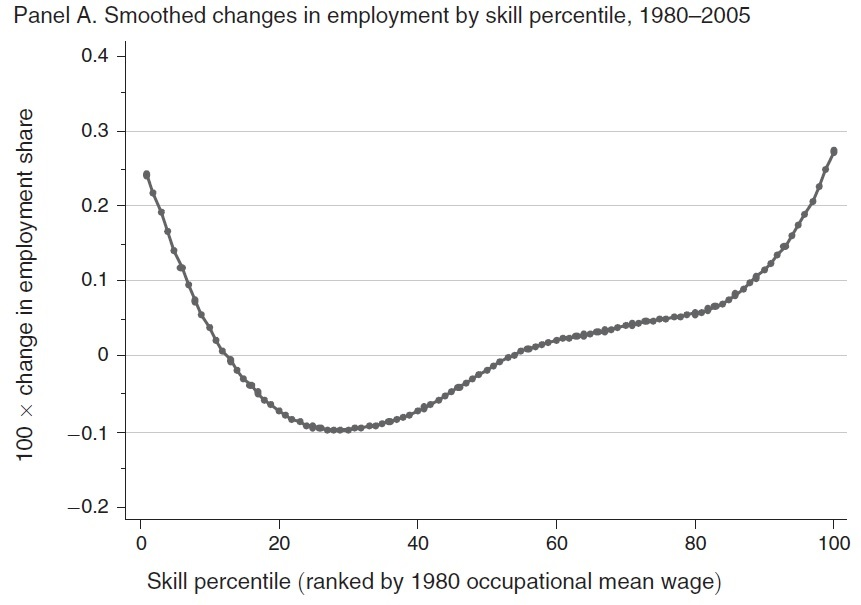
\includegraphics[width = 0.45\textwidth]{empl.jpg}

As evident by the figure it is especially the lower middle class and higher lower class that has lost jobs in the recent decades. A similar graph can be drawn for wage increases. Autor and Dorn proposes that the lower end increases are purely caused by the service sector, which has experienced rises in both wages and employment. By holding their wages constant at the 1980 model, it's possible to construct a graph without as much of an increase in the left tail. To do this the authors use a model where there is continuous technological progress in computing power, and multiple factors of production and sectors. From this they derive that when the elasticity of substitution between computers and routine labor is higher than the elasticity of substitution between goods and services in consumption there will be employment polarization. This happens as wages in routine labor drops, leading low skilled workers to apply for jobs in the service sector. Wage polarization follows as long as goods and services are at least weakly complementary. 
\\ \\
Alternative explanations include
\begin{itemize}
\item Offshoring of tasks, which displaces low-skilled workers into service jobs which are non offshorable. 
\item Rising incomes at the top of the wage distribution might increase the demand for services
\item Rising returns to skills for the college educated increase labor supply of these - substitute market for home based production (?) 
\end{itemize}

\subsubsection{Overeducation}
Some speculate if we invest to much in education relative to what the labor market can handle and demands. In this case workers will end up having jobs which require much lower skills than what they actually have acquired. Apart from the overproduction/underdemand reasons, a cause for over education could be search inefficiency, where the 'last' graduates simply would have to spend far to many resources finding a job in their trade.

Theres very little evidence, because measuring overeducation is not possible. Belfield suggests three ways we can potentially measure the degree of over-education
\begin{itemize}
\item Objectively: professional job analysts
\item Subjectively: through self reporting
\item The number of standard deviations above mean education in ones profession.
\end{itemize}
OECD however takes the approach of comparing actual schooling to what they call 'schooling needed'. To many highly educated individuals can have crowding out effects, in which case we should expect the unemployment rate of low-education types to increase as their jobs are taken by overqualified labor, and potentially also a decrease in the wage premium to college if supply outruns demand. 

What OECD find is that there are still high premiums for college, and there's no evidence of increased unemployment or supply-demand effects. Instead countries who had the fastest expansions in tertiary education also saw greater unemployment reductions for all.

Governments should be vary of intervening, as it depends on whether overeducation is permanent, temporary or part of a market response. Empirical findings suggest that overeducation tends to be temporary and helps unexperienced workers get a foothold in the labor market, without having any clear negative effects on productivity. 

\section{Part 9 - Educational financing}
\subsection{Lecture 17 - Educational financing}
There are many reasons why the government might want to be involved in the educational sector of the economy, including protection of minors, producing positive externalities and ensuring equality (of opportunity). Economic models usually assume that parents are altruistic in financing their childrens education, but what if this is not the case? We might be want the government to step in and ensure equal rights for such children. In relation to externalities evidence is scarce, the newest being the research done in crime reduction and health. 

There are also allocative arguments, some of which focus on the governments ability to circumvent credit constraints, while others focus on the redistributive aspects of education. Social scientists might also add that an educated population is necessary in a well functioning democracy, or even that common schools generate a common culture that is shared by all citizens. 

\subsubsection{The collective choice over public vs. private education}
We begin by studying the private demand for education, by constructing a 2-period model. In the first period agents invest in education, while in the second they consume and work. We assume the simplest HC production function we can
\begin{align*}
H_{it} = E_{it}
\end{align*}
and further that the earnings depend on ability and HC so
\begin{align*}
W_{it+1} = A_{it}^{\gamma}H_{it}^{\beta}, \quad \gamma, \beta \in [0,1]
\end{align*}
Utility is derived from their period 2 consumption as well as inheritance they can leave to their children
\begin{align*}
U_{it} = C_{it+1}^{\alpha}X_{it+1}^{1-\alpha}
\end{align*}
The budget constraint is $Y_{it+1}=C_{it+1}+X_{it+1}$ and we can then derive the indirect utility resulting from an optimal allocation of $C$, $Y$ and $X$ as 
\begin{align*}
V_i = \underbrace{\alpha^{\alpha}(1-\alpha)^{(1-\alpha)} }_{\equiv a} \cdot Y_{it+1}
\end{align*}
which show that ultimately the school regime will determine $Y_{it+1}$. 

\paragraph{Private school case} in the case of private schools the 2nd period income is given by 
\begin{align*}
Y_{it+1} = A_{it}^{\gamma}H_{it}^{\beta} + (X_{it} - E_{it})R
\end{align*}
where $R$ is the market interest rate. Agents then maximize their indirect utility given this budget constraint, that is 
\begin{align*}
\underset{E_{it}}{\text{max }} a Y_{it+1}
\end{align*}
which results in an optimal level of educational expenditures of 
\begin{align*}
E_{it}^{*priv} = \left[ \frac{\beta A_{it}^{\gamma}}{R} \right]^{\frac{1}{1-\beta}}
\end{align*}
Because schools are private each individual can freely choose his/hers optimal level of schooling. 

\paragraph{Public schooling} now lets instead say that each student gets a share of the total tax revenue, then it follow directly that 
\begin{align*}
E_{it}^{*pup} &= \frac{\tau_t \sum_{i=1}^n X_{it}}{n} \\
&= \tau_t \bar{X}_t
\end{align*}
This also changes income as taxes have to be paid, and there are no direct effects of $E_{it}$, so we get
\begin{align*}
Y_{it+1} = A_{it}^{\gamma}(\tau_t \bar{X}_t)^{\beta} + R \cdot X_{it}(1-\tau_t)
\end{align*}
this means the decision variable is the tax rate, and by maximizing as before, but now w.r.t $\tau_t$ we get the individuals optimal tax rate.
\begin{align*}
\tau_{it}^{*} = \frac{1}{\bar{X}_t} \left[ \frac{\beta A_{it}^{\gamma}}{R} \frac{\bar{X}_t}{X_{it}} \right]^{\frac{1}{1-\beta}}
\end{align*}
In society however there can only be one tax rate, so not everyone can get their optimal one, instead preferences generally are that those with high wealth would prefer a low tax rate, to avoid redistribution, while those with high abilities prefer a high tax rate to finance their education. To derive the overall tax rate lets consider two extreme cases.
\begin{itemize}
\item Egalitarian case - $A_{it}= A \ \forall i,t$
\item Elite case - $X_{it}= X_t = \bar{X}_t$
\end{itemize}

\paragraph{In the egalitarian case} the optimal tax rate is by definition only dependent on wealth - imagine the tax rate is decided by majority voting. In this case only the $\tau$ of the median voter can get a majority over all other proposals, so
\begin{align*}
\tau_{it}^{*vote} = \frac{1}{\bar{X}_t} \left[ \frac{\beta A^{\gamma}}{R} \frac{\bar{X}_t}{X_{t}^{median}} \right]^{\frac{1}{1-\beta}}
\end{align*}
in contrast a benevolent planner (who ignores all externalities) should choose 
\begin{align*}
\tau_{it}^{*planner} = \frac{1}{\bar{X}_t} \left[ \frac{\beta A^{\gamma}}{R}  \right]^{\frac{1}{1-\beta}}
\end{align*}
In societies where the income distribution is right skewed we will have $\bar{X}>X^{median}$ so in these cases the majority voting tax rate is larger than the one of a social planner, corresponding to over investment in education.
\begin{align*}
\tau_{it}^{*planner} < \tau_{it}^{*vote}
\end{align*}


\paragraph{In the elite case} the optimal tax rate depends only on abilities so 
\begin{align*}
\tau_{it}^{*vote} = \frac{1}{\bar{X}_t} \left[ \frac{\beta (A_{t}^{median})^{\gamma}}{R} \right]^{\frac{1}{1-\beta}}
\end{align*}
whereas the benevolent planner would prefer
\begin{align*}
\tau_{it}^{*planner} = \frac{1}{\bar{X}_t} \left[ \frac{\beta (\frac{1}{n} \sum_{t=1}^n A_{it} )^{\gamma}}{R} \right]^{\frac{1}{1-\beta}}
\end{align*}
So in the elite case which of the tax rates are highest depends on whether the average of $A$, $\frac{1}{n} \sum_{t=1}^n A_{it}$ weighted by $\gamma$ is higher or lower than the median $A_{t}^{median}$. Which is larger obviously depends both on the distribution of $A$ and on $\gamma$. Checchi assumed $\gamma = 1$ and a right skewed ability distribution, which leads to under investment in education. These assumptions are purely fictional, so in the end we cannot say much in the egalitarian case. 
\\ \\
So in the egalitarian case we had overinvestment, and in the elite case (maybe) underinvestment, but if we allow both $X$ and $A$ to vary it's still unlikely that we'll reach the optimal level of the planner, so majority control over how much to invest in education leads to inefficiency in investments. This can potentially lead to slower growth, but that is not to say we shouldn't have majority voting for education funds as there might be other concerns than growth to take into account. 

\subsubsection{Milton Friedman and the freedom of choice}
Friedman suggests we should consider the differences between publicly financed education and public provision of education - he suggests giving the financial aid to parents instead of directly to schools. In this way the government dictates both price and quantity. Such vouchers would increase the flexibility and allow parents to invest optimally in their children. Parents can only use their voucher for accredited schools and if the price is higher than the voucher they must pay the entire amount themselves. 

This scheme has some issues however, for example if parents are uninformed about school quality, from segregated communities and if travel expenses are non-negligible. Many solutions to the problems have been suggested.

Empirically we have very little evidence on the voucher system. In the US a small town implemented it, and found no gains in academic performance and high costs of implementation. 

\section{Papers discussed in the course}
This section will give brief overviews of the different papers is read throughout the course. The papers are separated into broad categories. Note that this list does not cover all articles, but only those i found relevant and/or are mentioned in the slides. There are papers mentioned above that are not included here.

\subsection{Credit constraints}
\paragraph{Checchi} say that if there are credit constraints we should expect more unequal countries (countries with high gini) to have lower enrollment rates. Similarly we should expect a positive relationship between public spending as  a share of GDP and enrollment. 

He tests this using cross country data on enrollment rates in primary, secondary and higher education. He only find significant results for secondary education, and stronger effects for girls across all groups. There is large explanatory power in the 1-below level of education (i.e. primary educ completion rates explain secondary education enrollment) suggesting a 'ratchet effect'. His results are criticized for being near-insignificant and his approach of using the gini. 


\paragraph{Belley Lochner} Compares two cohorts in the NLSY (National longitudinal survey of youth) to investigate the effects of family income on education. As measures of ability they use army test scores. They find that ability is more important in the bottom of the family income distribution, and that income has become more important from 79 to 97. While ability has become more important at the bottom, it has become less important at the top. 

\paragraph{Keane, Wolpin} find that students are tightly constrained in their credit options, but that these constraints doesn't matter much for completion rates, as reducing them would only increase labor supply while studying.

\paragraph{Carneiro, Heckman} find small gaps in college attainment by family income after controlling for ability. They say this is the case because ones financial situation at age 17 is the result of long run factors, so the constraints are binding far before it's time to send college applications. 

\subsection{Returns to human capital}
\paragraph{Duflo } studies the indosnesian INPRES program of school construction. He finds a very large return to a year of education by comparing children who attended before and after the new schools were constructed. 



\subsection{Skill formation over the life cycle}
\paragraph{The Perry preschool project} studies low ability children from disadvantaged homes. They randomly assign children to a treatment of two years of extra teaching, while their parents are also coached in socioeconomic factors. They find short term increases in cognitive abilities, but on factors like lifetime income and incarceration participants do much better than the control group. This suggests non-cognitive abilities are of great importance, which also shows from a comparison of parents valuation of 'good parenting' before and after the treatment - parents become significantly more aware of the importance of parenting.

\paragraph{Cunha, Heckman} build a many-period model with several periods of childhood to as best as possible match 'stylized facts' in economics of education. They include sensitive and critical periods of childhood, and derive both static and dynamic complementarity of investments and innate ability. 

\subsection{The production of human capital}
\paragraph{Hoxby} use natural variation in enrollment due to fluctuations of births as well as changes in minimum schooling laws. He finds no significant effect of class size in grades 4,6 and 8. 

\paragraph{Angrist, Lavy} Use an old Israeli rule that school classes must be divided in half when they exceed 40 students. They find significantly higher test scores in smaller classes in 4th and 5th grade. Their work suffers form problems with endogeneity of parents resudential choices, and because they only have variation between classes of size 20 and 40 (no lower). 

\paragraph{Calmar et al. (Aarhus RCT)} randomly assigns schools with money to hire extra co-teachers. Schools can either hire a co-teacher with or without a degree. There's generally no effect on math grades, only on reading grades. They find that co-teachers w.o. degrees are most helpful and helps children with low education parents the most. teachers with degrees help those with more able parents, and possibly the most disadvantaged in math.

\paragraph{Krueger} randomly assigns children to different class sizes and find small increases in performance. There is however evidence that enrollment rates to college increase for those in smaller classes. They had problems with parents withdrawing from the program if their children ended in large classes. 

\paragraph{Woesmann, West} look at the TIMSS data (Third International Maths and Science Study) across countries. Instead of using natural experiments they use school fixed effects to compare class sizes. They find that smaller classes are only beneficial for math grades in France and Iceland, while they matter for Science in Greece and Spain. In the remaining countries they find no effects. They further document that the four countries have lower than average performance, and educational expenditures. Greece and Iceland further pays teachers a below average salary. This could be evidence that class size only matters when teachers are not skilled to handle large classes.

\subsection{Evidence on intergenerational persistence ($\rho$)}

\paragraph{Mazumder} engages in a discussion of the size of $\rho$. Others have previously suggested that it's in the range of 0.2 to 0.35, but Mazumder claims these all have large issues because estimates of lifetime income are impossible to get precise. Using statistical techniques he estimates $\rho$ to be arrond 0.6. 

\paragraph{Björklund et al.} use Swedish adoptees to decompose genetics from environment in the intergenerational persistence equation. They find about equal contributions from biological parents and foster parents. Their study have been criticized as they assume that the transfer from bio- to foster parents happens at birth and assumes randomness in who gets which children. 

\paragraph{Twin studies} use twins to identify the causal returns to education, amongst other things. They are generally good studies but are critiqued for assuming that twins are identical - if they were they should also act the same - in other words, there's no guarantee that they don't vary on unobservables just because they're twins.  

\subsection{Crime and education}

\paragraph{Lochner, Moretti} use IV estimates on state specific changes in compulsory schooling laws to investigate the effect of education on crime. Their findings suggest large returns to education as it prevents crime. They use self-reported crime from the NLSY to avoid measurement errors, but have large problems with underreporting (for example on rape).

\paragraph{Lochner} builds a model in which agents trade of their gains and costs from working versus committing crime. They take up schooling beforehand, which alters their payout from the different activities. If people commit crimes they risk getting caught with a probability that is increasing in the amount of crime they commit. If that happens they must pay fines and spend time in jail. His model shows that how intitial HC affects investments in education will depend on how skilled the individual is at crime, compared to learning. 

\subsection{Health and education}
\paragraph{Lleras, Muney} use three census cohorts, each separated by one decade to calculate death rates between them. They face some problems with imprecise death rate calculations, giving them negative death rates for some ages, but continue nonetheless. They then use state specific changes in compulsory schooling laws from 1915-1939 as a quasi-experiment, to investigate of schooling matters for lifetime through a regression discontinuity setup. They find significant results for the 10-year death rate on a number of regressions. Using IV they get higher estimates, suggesting a concave relationship between education and health. Years of compulsory schooling also provides significant results. 

\paragraph{Grossman} Builds a dynamic model where health is an investment good, and affects the time of life, thereby altering the expected return to education.

\paragraph{The Rand health insurance experiment} randomly assigned US individuals to one of five specifically designed health insurance plans. They found little effect from health insurance on health, except for small subgroups of their population. The general conclusion was that increasing health insurance would be \textit{less} cost effective than effective educational interventions. 

\subsection{Growth and education}

\paragraph{Barro} finds results indicating that extra schooling does increase the GDP growth rate.

\paragraph{Behrman, Birdsall} Criticizes previous research into the relationship between growth and education for not taking into account the differences in the quality of education. They say quality is at least as important as quantity. 

\paragraph{Hanushek,(Kimko/Wössmann)} use international test data as proxy for the quality of education, they find significant and large results of quality of education on growth compared to the effect of quantity of education. Their approach makes years of schooling insignificant.

\subsection{Polarization of the labor market}
\paragraph{Autor, Dorn} observe a large increase in wage inequality. Unlike what the ordinary SBTC hypothesis would say, the changes are not monotone, as both employment and wages at the lowest paying jobs have also increased. They say service jobs account for the large increase in low-wage jobs. They construct a model to explain the phenomena, and finds that 
\begin{itemize}
\item \textit{employment polarization} happens when the elasticity of substitution between computers and routine labor (in production) is larger than the elasticity of substitution between goods and services (in consumption).
\item \textit{wage polarization} happens if goods and services (in consumption) are at least weakly complementary. 
\end{itemize}

% \section{Old exams and tests}
% \subsection{2013 winter exam}
% \paragraph{Question 1} In a situation with mass layoffs especially among young workers, many different things happen. First of we would assume that human capital depreciates to some extent, which automatically reduce the future productivity of those who are unemployed. How much human capital depreciates is difficult to say, and there are special kinds of depreciation which aren't continuous. Specifically if many of those who are laid of have received on-the-job training specifically tailored for the company they were employed in will experience sharp declines in the productive value of their human capital. How large this effect is depends heavily on the degree of specialization within different sectors, with those who have been employed in very specialized sectors loosing the most productive value. Those with completely general skills acquired through OTJ training will not experience any discontinuity in their decline of human capital. 

% It's possible that those with specialized training loose little in terms of wages, as they would not have been in a position to negotiate high wages before their firing. This is because in the case of specialized training workers outside options stay the same since their skills are only productive in the company they're currently at, so if they regain employment at their previous outside option wage, it might not be very different from what they earned before. 
% \\ \\
% How their future wages evolve is unclear. Assuming an individual is young and not credit constrained to the extend where school is unfordable, the Ben Porath model predicts the agent taking up more school, as the relationship between current and future wages have increased. This in turn increases the human capital of the agent, who can then later earn her increased marginal product. This speaks in favor of increasing wages in the long run. Extending the concept of dynamic complementarity to cover OTJ training is further in favor of higher wages with a more concave profile, as future employers will know that the additional education acquired during the crisis increases the return to further investments, they might therefore allow for additional general OTJ training, paid for in the beginning through the wages of the employer, but later on employed to increase wages. 

% Oppositely one might speculate if those who manage to keep a job through the crisis will be able to use this as a signal to maintain high wages although they miss out on additional education. 

% For older workers going to school makes little sense as they wont have enough time left on the labor market to reap the benefits from newly earned education. They will therefore must likely see a decrease in their wages which never recover. 
% \\ \\
% Employers are mildly affected at the beginning, as they only loose employees who 1) they fire themselves and 2) experience slow wage growth and therefore pursue more education. As the crisis ends however they will be able to hire well educated workers.



% \paragraph{Question 2} A sharp rise in unemployment will most likely increase the demand for education. Those who loose their job will most likely see their potential income decline rapidly after being fired, as finding a new job will be near impossible. If they anticipate a coming economic upturn this will imply that their potential wages today are much lower than what they can expect to get in the future. This will drive up school attendance in accordance with the $\frac{\beta_{t+1}}{\beta}$ term in the expression for optimal schooling of the Ben-Porath model. The increase in demand will be decreasing in age, as those who are nearing their end on the labor market doesn't have time to reap the benefits of increased education. 

% Instead the older generation will be likely to spend savings or gain employment at a lower wage. If the younger generations have managed to save enough they can take up school again, but if savings are insufficient many of them might find themselves credit constrained, especially considering the banks tendency to decrease loaning. In this case they will get a suboptimal level of schooling.

% All age groups will be tempted to take up more education as a result of the reduced opportunity costs, except for those who are so old that $W_{t+1}=0$ i.e. those who will retire. To them there is no gain whatsoever from educating themselves. 
% \\ \\
% A group not yet discussed is those without previous labor experience, namely children. They aren't in a position to choose how much education to get themselves, but parents of children might react to the sudden loss of jobs as well. Parents themselves are subject to the layoffs, so they will (at least at an aggregate level) loose income, thereby their marginal utility of consumption increases and they will reduce spending on their childrens education accordingly. More parents will also become credit constrained, meaning that even more children doesn't reach their optimal level of education.


% \paragraph{Question 3} Wages of newly graduated, relative to previous cohorts. If the newly graduated have received less schooling as a result of the drop in parents income, they will have a lower level of human capital, compared to their older coworkers who spend the crisis acquiring additional HC. This alone puts them at a worse position in terms of wages than the older generations. Instead they will not have spend any time on unemployment, making the net effect difficult to tell. 

% New entrants on the job market may also benefit from pooling equilibria in signaling games, as they will potentially get pooled with significantly more educated workers - however firms might adjust hiring strategies accordingly, for example to assume that anyone without previous experience is 'low ability' compared to someone with the same degree and experienced. In this way firms can sort workers into groups of those with increased 'crisis-education' and those without it. However if firms cannot tell apart graduates and those who attended university as a result of reduced opportunity costs, thing will be different. In this case those who were laid of and took up education is likely to be 1) previously credit constrained or 2) of lower ability. So assuming that those who were previously credit constrained don't have their constraints loosened by a crisis, the total population of graduates will on average be of lower ability. Therefore firms will reduce the wage premium for education, to account for the surge of low-ability high-education applicants. 

% supply and demand in a situation with abnormally many highly educated will also lower the returns to education, and might lead to overeducation where some of those with newly earned higher education degrees are unable to find jobs that match their qualifications. This in turn would also lower the wage premium to education.

% the quality argument: if governments cut spending, this might affect school quality, although this is entirely dependent on the setting, as empirical evidence for a spending-quality relation is inconclusive and points to the most important thing being how resources are allocated within the educational sector. So we could imagine budget cuts being coupled with efficiency enhancing policies, thereby offsetting the negative effect on quality. 


% \paragraph{Question 4} Within families the strictly economic arguments point towards lower education of children, i.e. as mentioned previously because of dropping family incomes and the resulting changes in allocation and credit constraints. If the expected return to education itself changes is unclear - this will largely depend on how wages develop in the future, and this is unclear. Factors going into the future wage is demographical dynamics, i.e. when will the old workers who didn't take extra education leave the labor market (this will increase the general educational level on the market substantially and thereby drive down wages for highly educated), does certain sectors get set back more than others (possibly sectors with lots of specific OTJ training will take a long time to recover, making it possible for new entrants on the labor market in these sectors to compete on equal footing).

% The model by Cunha \& heckman can be used to argue that graduates will vary more in their human capital levels. To illustrate imagine that the recession strikes at time $t$ and it makes parents more credit constrained. Then those children who are in sensitive or critical periods will suffer long term reductions in their gains from education, while children only a few years older are affected substantially less - which would cause high variation in the abilities of the following years of graduates. 
% \\ \\
% There are however substantial evidence that socioeconomic factors like patience play a large role in the attainment of early education. For example the Perry preschool project suggests that early childhood intervention and parents attitude towards parenting can substantially improve lifetime outcomes of disadvantaged children. If layoffs improve parents time to engage with their children this might even be beneficial to their educational success.

% \paragraph{Question 5} The previous arguments are not all in accordance, but can roughly be summed up as 
% \begin{itemize}
% \item Current workers take up more education, unless they're nearing retirement.
% \item Specialized sectors loose the gains from employer-employee benefits established through specific OTJ training.
% \item Children (might) get less education because of credit constraints and lower family income.
% \item ... but they might also stay in school longer
% \item Job markets are structurally altered, amongst others because of new signaling effects.
% \end{itemize}
% So as the crisis ends we can expect sectors with a high degree of general knowledge to grow again, driven by the high educational level of those who took the opportunity of getting education while unemployed. At the same time this will act to push older generations out of the labor market as they're bound to slowly loose jobs to more highly educated applicants, potentially straining the Greek public economy. Specialized sectors will be slow to regain their pace, but this on the other hand gives new entrants in the labor market an easier chance of getting in, as many positions will open at once. 
% \\ \\
% New high ability graduates will find themselves in a difficult position, as they will compete with low ability types who acquired education during the crisis, potentially without a way to distinct themselves, thus ending in a pooling equilibrium. They might also face problems with over-education, which ultimately means resources have been wasted on education which wasn't necessary. 

% How the job market changes on a structural level is difficult to say, but it is likely that changes will happen, potentially in a direction where new specialized sectors emerge, and old ones disappear. How the (likely) increase in educational attainment affects growth is hard to say. Behrman \& Birdsall seem to find that quality of education is just as important as quantity when it comes to education induced growth, and thus how this pans out depends entirely on how the educational system fares through the crisis. 

% \subsection{2014 winter exam}

% \paragraph{Question 1 - private over public schools} 
% Why parent choose to send their children to private school can be explained in a number of ways. The choice can be considered to reside either with the pupil or the parents, and in some cases which perspective is used doesn't matter much. 

% First of all private schools might simply be more productive than public schools, due to a number of factors. Although this could come down to resources there is little evidence that spending on education itself raises students abilities - see for example Denmark, which spends large sums, but ranks relatively low in international student tests. Several researchers, including  Instead evidence points to several factors being important. 

% Calmar et al. conducted a RCT Denmark to show that class size (or at least teachers per student matters) they allow primary schools to hire extra teachers either with or without a degree, and find that this increases students test scores in reading. They find differences how additional teachers help, on the basis of parental background. If German private schools pursue this idea of allocating more teachers to each classroom, they might simply be more productive than public schools. 

% Cortez et al. find some gains to student achievement simply from having good teachers, so if private schools can show high average teacher value added, this might incentivize parents to send their children to private schools. This is in line with the macro evidence by Berhman and Birdsall who find high returns to the 'quality' of education between countries. 

% There's also the possibility that private schools provide more targeted aid for low-scoring students, comparable to that of the Perry Preschool project, which showed long term gains in terms of income and health for participants even though their cognitive gains were short lasting. 
% \\ \\
% It's often implicit in the discussion about private schools that they are more expensive than public schools (which is as far as i know free in Germany). If this is the case, parents might have other motives to send their children to private school than the purely productive ones. 

% First of if we assume that abilities are inherited to some extent, the price of private schools can function as a cutoff for low ability students if credit constraints are primarily present among the poorer families. In this case there might be signal value to private school as graduates will be more likely to be high ability than their peer graduates from public school.

% 'high-skill segregation' might also give rise to peer effects, although how large these are is uncertain. Carell, Fullerton and West randomly assigned groups in the US army, and found that mixed-ability groups didn't increase gains to those with high ability, but reduced learning outcomes for the low ability types. 
% \\ \\
% In the Becker Tomes model we can explain a shift to private schools through a number of mechanisms, first of if parents are very altruistic and they believe private schools to have higher returns, they will be willing to reduce their own consumption to finance private school attendance for their children. In this case children from every parental background should attend private school more (assuming credit constraints are insignificant).
% \\ \\
% It's also an option that parents are aware of the changes in the labor market described by the SBTC hypothesis, and react to this by investing more in specialized education early on. This would benefit students through the mechanism of dynamic complementarity described by Cunha and Heckman - as investments raise abilities in period t, and abilities raise the productivity of investments in later period, these two compliment each other, and so adding an element of specialized knowledge to this theory would predict large returns to those with early specializations in high-technology jobs.  


% \paragraph{Question 2}
% That people choose to attend private schools could suggest that Germany is in a situation somewhat like the extreme of 'equal wealth' where the median voter dictates a level of investments lower than the optimal amount (assuming the ability distribution is right skewed). In this case those attending private school are likely to be the high ability voters who would prefer more education than what is provided through the educational system. 

% When students start leaving the public schools the voter decided expenditures on education stays constant, but the number of students drop, thereby leading to higher expenditures per student in the public schools. This should in itself increase the quality of public schools, as long as they follow the strategies proved to work (i.e. reduced class sizes and early intervention). 
% \\ \\
% An open question is how the voting behavior of those attending private schools changes. If regulation allows every student a fixed amount of money to spend on education in either public or private schools, their behavior is likely to stay the same, and the optimal voting tax rate stays constant. If however students at private schools has to pay the entire price themselves, they will probably vote for 0 expenditures towards public education, thereby reducing the median voter tax rate, and offsetting the effect of increased per student expenditures in the public sector. 


% \paragraph{Question 3 - no right to reject}
% Prohibiting schools from excluding students from poor backgrounds would, if private schools are truely more productive than public schools, increase attendance by low ability students (as wells as high-ability, low family income students) in private schools, thereby making the student body resemble that of a fully public school system. Since ability is inherited this would also reduce the average student ability at private schools and make them resemble public school more. 

% If private schools work as a signal, the separation that previously occurred because low income families couldn't afford private schools would disappear, thus removing any benefits to those with high income parents derived from attending private school.

% The above assumes that children of any parental background are equal in their previous achievements and abilities, but c.f. the Perry preschool project and Cunha and Heckmans model of dynamic complementarity this might not be the case. Specifically children from low income families, are due to inheritability likely to have lower innate ablities, and therefore gain less from additional education than other students. To compensate for the lower innate ability children from a low income background might benefit relatively more from non-cognitive schooling than their high ability peers. 

% If this is the case we can imagine a sorting happening where high-income parents still send their children to private school, knowing that the low-ability students have lower gains from cognitive education and therefore send their children to public school. This requires that the school system learns from the behavior of parents, that they should supply either cognitive or non-cognitive training.
% This mechanism can also be brought about by the private schools by hiring high-skilled co teachers, who have been shown to predominantly benefit children of higher income families. 

% \paragraph{Question 4}
% Entrance tests are essentially restrictions for those who are a) low ability or b) have had low quality (and/or quality) non-cognitive or cognitive training previously to applying for school. 

% Assuming first that human capital is at all productive, these kinds of entrance exams might be efficient if those who are rejected are predominantly low-ability and there are significant peer effects from 'skill segregation'. As mentioned Carell, Fullerton and West find negative peer effects from groups that are extreme in their composition, which could be interpreted as weak evidence that schools with a broad composition of students in terms of background can reduce learning outcomes. Jackson also finds some evidence for peer effects from being with high ability peers, but fail to show any non-linearities in the effects, suggesting that 'rearranging' student compositions wont increase overall skill attainment. Thus whether entrance tests will improve overall educational attainment in society is dubious, but Jacksons results suggests that entrance tests migh benefit those who are admitted to the school. 

% \paragraph{Question 5}
% A country which previously had no merit based scholarships, but then moves to a system where private schools and universities provide such scholarships is comparable to a case where there is positive covariance between skills and the supply of education for the most able. 

% In the simplest, and most unrealistic, case there is only one supply and one demand for education (equality of outcomes). Introducing a new supply that is higher and only achievable by the most highly skilled would only be used by those who enjoy going to school as it implies both larger expenses to education and a lower marginal productivity from the investments, which entails a lower wage.

% We can instead consider the case where there is equality of opportunity except from for those with very high abilities - that is those with high demands for education. This corresponds to a situation with many demand curves, but only two supply curves. This case is somewhat similar to the case of variations in both supply and demand, but stylized as there are only two types of supply - one for ordinary people and one for those with high abilities. In this setting those with high enough abilities will jump to the new higher demand, thus taking up more education while earning lower or the same wages as they could have if their supply was lower. This will reduce inequality as it clusters incomes around the cutoff for merit programs.  

% \paragraph{Question 6}
% There are many ways to study if private schools actually are more productive than their public counterparts, ideally we would like to construct a randomized control trial, but lower on the ladder are things like regression discontinuity designs, natural experiments and IV estimates.

% \begin{itemize}
% \item Assuming funds for conducting a RCT is available, we would still have to be cautionary with how we proceeded, as randomly admitting children to either private- or public school would make such things as peer effects disappear, thus if we used this technique we could only measure the direct effects from the school choice. Furthermore the ethics of such programs are questionable as it could assign individuals to bad education which shapes the rest of their lives.
% \item A natural experiment would require us to observe a situation where people were randomly assigned to either public or private school, or randomly were switched between them. How this might happen is difficult to say, but with sufficient data it might be possible to study a subsample of students experiencing school closings with only one alternative school option. 
% \item Using IV we need to devise of an instrument that correlates with school choice, but not with background characteristics that might influence school choice directly or indirectly. One example could be a metric for the relative distance to the nearest public- or private school. This should correlate with the choice of school (people tend to choose what's closer) but not with family background or abilities. 
% \end{itemize}

% \subsection{2015 Winter}

% \paragraph{Question 1}
% \begin{itemize}
% \item[a)] Ben porath - lower E gives lower H gives lower S, reduces inequality, lower attainment

% Becker Tomes (less relevant since parents dont decide to got to uni) - lower s will reduce the returns to investing, but also increase the indirect MU of education as it increases childrens earnings more.  -> Ambiguity -> assume investment effects are strongest so x goes down ... lower attainment 
% \item[b)] Lower Expenditures will be worst for the high skill students - consider the interior function AHE - holding, A,E constant high skill students have the larges slope from changes in investments. So as well as benefiting most, they also stand to loose the most. Changes would reduce inequality as public expenditure is multiplicative with ability in the ben porath model, i.e. low ability students can still benefit from the lower expenditures, while those wilt high ability needs more to get optimal schooling. 
% \item[c)] Literature on ressource use - little effect from direct spending, seems usage is more important. Calmar et al -> class size (more like active instruction time) is important - comparable to TA classes, these can have a big impact. Dobbie Fryer -> no effects from traditional measures, identifies some keys to good outcomes of education: 'frequent feedback', instruction time, tutoring - all of which are high cost tools (uses charter schools, not high external validity). Jackson - TVA, which can be argued to decline has large effects on non-cognitive behavior (uses it to predict college attendance - not necessarily the same after going).

% Woesmann and West - Find effect in few countries by using TIMSS data, but suffers from a weak instrument.  



% \end{itemize}

% \paragraph{Question 2}
% \begin{itemize}
% \item[a)] In Becker Tomes it comes down to credit constraints, as a reduction in grants would increase the amount needed for borrowing (holding a constant) parents would fill out some of the gap, but not the whole thing (indirect MU equal to return) those who become constrained will not get optimal schooling, i.e. a reduction of attainment, because more doesn't achieve optimal level. 

% Literature:
% Keane Wolpin - students are tightly constrained, but are not affected by them, so loosening constraints would only lower labor supply and increase consumption -> in our case tightening credit constaints would increase labor supply and decrease consumption.

% Checchi - finds evidence of credit constraints in macro data using the gini coefficient and education attainment rates to show credit constraints.

% Carneiro, Heckman - finds no evidence of credit constraints after controlling for ability at age 17 - believes constraints make themselves binding far earlier than at application time. 
% \end{itemize}

% \paragraph{Question 3}
% \begin{itemize}
% \item[a)] First of all - it produces human capital, and is not purely signaling. otherwise it would be inefficient to let people educate themselves. Secondly There are positive externalities from education - i.e. a democratic people or similar, and people are sometimes not able to invest the amount they want in education. 
% Danish case - a more ideological quest for equality of opportunity and/or people consider private and public investment near-perfect substitutes in denmark.

% \item[b)] It could be that there are significantly greater gains from educ in Denmark (unlikely). Welath is distributed evenly, by the median voter theorem, leads to overinvestment in education if ability is right skewed. 

% \end{itemize}

% \subsection{Re-exam 2015 winter}

% \paragraph{Question 1}
% \begin{itemize}
% \item[a)] In Ben Porath higher educational attainment can be explained by 
% \begin{itemize}
% \item[$\frac{\beta_{t+1}}{\beta}$ (+)] If the relative wages as adults, compared to as youths are larger for women than for men, this can lead to a increase in the attainment of education for women.
% \item[$\alpha$ (+)] If the production of Human capital in women is more effective than in men, they might earn more education than men.
% \item[$\gamma$ (-)] If the direct costs of education are lower for women, they will take up more education than men.
% \item[$\rho$ (-)] If women discount the future less heavily i.e. are more foresighted, they will take up more education, as they have greater preferences for future income. 
% \item[$E_{it}$ (+)] If the ressources invested in womens education are greater than those invested in mens education, womens education becomes more productive and they take up more of it. 
% \item[$A_i$ (+)] If women carry more innate abilities they will take up more education.
% \end{itemize}

% Some suggest that the girls production of human capital in the early years is higher than that of boys (they're for example better at paying attention) this effect could carry on into adulthood d.f. Cunha, Heckmans model with dynamic complementarity. Along the same line, girls could be more patient than men, leading them to put more weight on future income. Concerning abilities it's difficult to tell if girls are born with more innate ability than boys, but if they do the differences are probably small, and it's more likely that boys and girls are identical in innate abilities at birth. 

% Among the less likely explanations are that spending in womens education are higher than in mens. Also since wages by job are similar for men and women this is also an unlikely situation. The gender 'wage gap' seems to be primarily caused by a 'sector segregation' between the genders, and if anything speaks to womens wages being lower in the future than mens. The direct costs of education are also approximately identical between the genders.
% \\ \\
% Although not mentioned by the question signaling could play a role as well. Specifically if employers require greater achievement from women to believe they are high-ability those girls who were very able would want to take up additional education to avoid being pooled in with the low ability types. 

% \item[b)] The model by Becker Tomes both exists with and without credit constraints. Furthermore in incorporates an element of inheritability. If we assume away credit constraints, parents achieve the optimal level of schooling for their children by borrowing until the interest rate is equal to the marginal return of investing in their children. In this setting girls would therefore get more education than boys if 1) the interest rate faced by girls is lower than the one faced by boys or 2) girls marginal return to investments in education are lower for those of boys, so that they will need more education to reach the same level of return as the interest rate. This is contrary to the Ben Porath model, where explanations pointed to girls having larger returns. 

% In the credit constrained case parents balance their own marginal utility of consumption with the indirect marginal utility of investments in their childs education (which is a function of private- and public investments, as well as endowments). The indirect utility is weighted with a parameter 'a' measuring the degree of 'altruism' of the parents. If parents of girls are more altruistic towards their children, this would lead them to reduce own consumption in favor of investments and thereby increasing the educational level of girls compared to boys. Credit constraints might also play a part, specifically imagine a situation where parents of boys are more often credit constrained, but expenditures and altruism are otherwise identically distributed. This could be caused by different degrees of ability inheritance between the genders. If boys show a greater degree of mean reversion in terms of innate abilities they will A) have rich parents, who can easily finance their relatively low demand for education or B) have relatively poor parents, who are credit constrained from financing their high demand for education. If this was the case girls would in most cases get educated to their optimal level, but only boys with endowments that were at or below the level of their parents would be able to get the education they demand, effectively making very high ability boys get to little education. 

% \item[c)] Depending on the cause of the educational gap solutions will be different. If the reason for the gap is simply that boys are on average of lower ability than girls, it might be effective to do nothing at all. In the models with perfect capital markets this is more likely to be the case, as they don't assume any restrictions on agents abilities to finance education. If the differences was due to credit constraints it could be efficient to alleviate these trough transfers or special schemes, but Hoxby and Carneiro, Heckman both find that loosening credit constraints will not increase education. 

% Checchi finds evidence for credit constraints in macro data. His hypothesis is that if credit constraints are present predominantly in low income families, unequal societies should have lower admission rates. His results are inconclusive for primary and tertiary education, but forsecondary schools he find evidence that this is the case, leading him to the conclussion that credit constraints are present and causes lower admission for poor students.  

% Belley, Lochner on the other hand suggest credit constraints could be binding for especially the lower income level based on a comparison of two cohorts of US citizens.
% \end{itemize}

% \paragraph{Question 2}

% Measuring returns to education is difficult but a number of methods have been proposed. One of the most tempting ways is to use twin studies, as twins are (at least superficially) identical on a broad range of characteristics that are typically difficult to observe. These studies however face a serious critique as they hinge on the idea that twins are identical, but as critics have pointed out this cannot be the case if twins choose different educations. 

% The most direct way of measuring the returns to education is though the Mincer earnings function, which is a good benchmark to compare other methods again. The mincer equation is however not causal and requires the imposition of strict assumptions to be give estimates of the internal rate of return on investments in education.

% Duflo have used the Indonesian school construction project INPRESS as a natural experiment and found large returns to education. More generally the use of natural experiments can also be used in the context of compulsory schooling laws to investigate returns to a year of education. Sometimes IV estimates are used in conjunction with these. Valid and relevant instruments have the strength of isolating the pure effect of x on y, but only give the effect of the instrument of the sample that is effected, thus estimates cannot be considered average effects in the whole populations. One widely used instrument is that of distance to college, as it varies with attendance to college, but can reasonably be claimed to not covary with unobservables. Whether this is completely true is however not set in stone, we could easily imagine a scenario where schools are build in rich/high-endowment neighborhoods and or that highly able parents move closer to good schools. 


% \paragraph{Question 3}
% There is a lot of literature studying the production of skills in school, and in many cases comparing results show that the current evidence is inconclusive. For boosting the completion rates and grades of boys evidence could be

% Dobbie, Fryer who investigate the effects of traditional measures such as class size or teacher qualifications/wages using lottery admissions to NYC charter schools and find that these variables generally are poor at determining students grades. They suggest instead that factors such as teacher feedback, instructional time and high dosage tutoring give the greatest results. 

% Calmar et al. who have run a RCT based in Aarhus, denmark to study the effects of coteachers, and find that these are generally beneficial for reading grades but less so for math. They find that coteachers without degrees are generally most helpful for children of low income homes, but also that teachers with degree can help with math scores and children from more advantaged homes. 

% The Perry preschool project indicate long term effects primarily working through non-cognitive effects for early childhood intervention. This is in line with the model by Cunha, Heckman where dynamic complementarity makes investments in the early childhood more rewarding in terms of returns to education. 

% From research in Maimonides rule there is some evidence that class sizes matter, but this research suffers from the fact that the rule only generates variation between class sizes of 20 and 40, with no classes below this level. 

% Thus from an economic standpoint it would be preferable to invest the extra funds in early childhood programs if the goal is to encourage more boys to attend school. If instead the target for policy is to increase the performance of boys already in school and/or prevent dropouts evidence is less clear, but the recommendations of Dobbie, Fryer and the results from Calmar et al. would be a good starting point - increased teacher feedback, and tutoring for disavantaged boys, combined with the introduction of co-teachers would be a good way to spend the public funds. 




\end{multicols}

%\end{spacing}
\end{document}